\documentclass[10pt]{article}
\usepackage[left=0.8in,right=0.8in,bottom=0.5in,top=0.5in]{geometry}
\geometry{a4paper}
\usepackage[parfill]{parskip}    % Activate to begin paragraphs with an empty line rather than an indent
\usepackage{graphicx}
\usepackage{xcolor}
\usepackage{hyperref}
\usepackage{titling}
\usepackage[small,compact]{titlesec}
\usepackage[toc,page]{appendix}

\usepackage{listings}
\usepackage{pgfplots}
\usepackage{adjustbox}
\usepackage{float}
\usepackage{subcaption}
\usepackage{pgffor}
\usepackage{expl3}
\usepackage{xparse}
\usepackage{xfp}
\usetikzlibrary{fit}
\usetikzlibrary{positioning}


\usepackage{amsmath,amssymb}
\DeclareGraphicsRule{.tif}{png}{.png}{`convert #1 `dirname #1`/`basename #1 .tif`.png}



\newcommand\courseName{Language-Based Security}
\newcommand\courseNameAbbrv{LBS}
\newcommand\courseYear{2023}
\newcommand\courseAndYear{\courseNameAbbrv-\courseYear}
\newcommand\reportKind{Exam Report}

\newcommand\groupNumber[1]{
  \makeatletter
  \def\@courseGroupNumber{#1}
  \makeatother
}

\pretitle{\begin{flushright} \bfseries  \large \courseAndYear: \reportKind \end{flushright}   \begin{flushleft}
\bfseries \LARGE}
\posttitle{\par\end{flushleft}\vskip 0.5em}

\preauthor{
\begin{flushleft}
\large \lineskip 0.5em%
\bfseries
\makeatletter Group \@courseGroupNumber \\ \makeatother
\begin{tabular}[t]{@{}l}}
\postauthor{\end{tabular}\par\end{flushleft}}

\predate{\begin{flushleft}\bfseries \large}
\postdate{\par\end{flushleft}}

\usepackage{listings}
\usepackage{pgfplots}
\usepackage{adjustbox}
\usepackage{float}
\usepackage{subcaption}
\usepackage{pgffor}
\usepackage{expl3}
\usepackage{xparse}
\usepackage{xfp}

\newcommand\todo[1]{\textcolor{red}{TODO: #1}}

\pgfplotsset{compat=1.12}

\definecolor{mGreen}{rgb}{0,0.6,0}
\definecolor{mGray}{rgb}{0.5,0.5,0.5}
\definecolor{mPurple}{rgb}{0.58,0,0.82}
\definecolor{backgroundColour}{rgb}{0.95,0.95,0.92}

\definecolor{firstCol}{HTML}{332288}
\definecolor{secondCol}{HTML}{117733}
\definecolor{thirdCol}{HTML}{44AA99}
\definecolor{fourthCol}{HTML}{88CCEE}
\definecolor{fifthCol}{HTML}{DDCC77}
\definecolor{sixthCol}{HTML}{DD2255}

\lstdefinestyle{defstyle}{
    backgroundcolor=\color{backgroundColour},   
    commentstyle=\color{mGreen},
    keywordstyle=\color{magenta},
    numberstyle=\tiny\color{mGray},
    stringstyle=\color{mPurple},
    basicstyle=\footnotesize,
    breakatwhitespace=false,         
    breaklines=true,                 
    captionpos=b,                    
    keepspaces=true,                 
    numbers=left,                    
    numbersep=5pt,                  
    showspaces=false,                
    showstringspaces=false,
    showtabs=false,                  
    tabsize=2
}

\newsavebox{\mybox}

\ExplSyntaxOn
\cs_new:Npn \__afp_ismember_loop:Nnw #1#2#3,
  {
    \quark_if_recursion_tail_stop_do:nn {#3}
      { \prg_return_false: }
    #1 {#2} {#3}
      { \use_i_delimit_by_q_recursion_stop:nw { \prg_return_true: } }
      { \__afp_ismember_loop:Nnw #1 {#2} }
  }
\prg_new_conditional:Npnn \afp_int_ismember:nn #1#2 { p, T, F, TF }
  {
    \__afp_ismember_loop:Nnw \__afp_int_isequal:nnTF {#1} #2 ,
    \q_recursion_tail , \q_recursion_stop
  }
\prg_new_conditional:Npnn \__afp_int_isequal:nn #1#2 { p, T, F, TF }
  {
    \int_compare:nNnTF {#1} = {#2}
      { \prg_return_true: }
      { \prg_return_false: }
  }
\NewExpandableDocumentCommand { \IncludeExperimentResults } { m m }
  {
    \foreach \x in {1,...,#1} {
        \noindent\bool_if:NF { \afp_int_ismember_p:nn {\x} {#2} } {\input{generated_latex/prog\x.tex}}
    }
  }
\ExplSyntaxOff
\usepackage[authoryear]{natbib}

\title{
  Optimizing Away Security in C
}

\groupNumber{10}
\author{Anders B. Clausen \and Johan T. Degn \and Jonathan S. Eilath}

\begin{document}
\maketitle
\thispagestyle{empty}

\todo{Add short guide to read data plots}
\todo{We can probably add "what compile flags are dangerous" to contributions}
\todo{We can analyze md=12 for example, but not show it in the report. THIS IS DONE?}
\todo{We should only have a few analysis results in the appendix since including all would be overwhelming!}
\todo{OptiFuzz might be used in a CI pipeline to detect timing vulnerabilities automatically. MENTION THIS?}

\section*{Abstract}
\todo{After the paper is done}

\section{Introduction}
The C programming language is one of the most widely used programming languages in the world. 
It is used in a wide variety of applications, ranging from embedded systems to cryptographic libraries. 
However, C is also notorious for lacking security guarantees.
Security-related issues in programs written in C stem from both the programmer, but also from the compiler.

The problem with security issues introduced by the compiler is especially prevalent in the context of timing attacks on cryptographic algorithms. 
Developers try to mitigate timing attacks by writing constant-time code -- code where the execution time is independent of the input.
However, the compiler may introduce timing leaks by optimizing away the constant-time code.
In a recent study \citep{developer-survey-timing-attacks}, it was shown that the vast majority of developers of cryptographic libraries rely on constant-time code practices that in theory result in constant-time code, but may be vulnerable after compilation.

The issue of timing vulnerabilities introduced by compilers is well-known in the community.
Several proposals have been made to mitigate the issue \citep{what-you-c, dudect, fact, verified-constant-time-c-comiler}.
However, the problem persists and to the best of our knowledge, no study has quantified the issue of timing vulnerabilities introduced by compilers.

In this paper, we try to quantify the issue of timing vulnerabilities introduced by the two most popular C compilers, gcc\footnote{\url{https://gcc.gnu.org/}.} and clang\footnote{\url{https://clang.llvm.org/}.}.
We do this by implementing a tool, OptiFuzz, that generates, analyzes and fuzzes random C programs.
For simplicity, the generated programs are limited to only containing non-branching arithmetic, logical and comparison operations.
Also \texttt{/} and \texttt{\%} are avoided, to mitigate division-by-zero errors.
We investigate what optimization flags are responsible for introducing timing leaks and compare them.
Finally, we discuss how the issue of timing vulnerabilities introduced by the compiler can be mitigated by using language-based security techniques.

\subsection{Related Work}
The issue of timing vulnerabilities introduced by the clang C compiler across different versions has been researched by Simon et. al. \citep{what-you-c}. 
Several studies have investigated potential solutions to the issue, including using constant-time branching instructions \citep{what-you-c}, using black-box testing software \citep{dudect}, domain-specific languages \citep{fact}, and notably a verified constant-time C compiler has been developed \citep{verified-constant-time-c-comiler}.

\subsection{Contributions}
We provide a quantitative analysis of timing vulnerabilities introduced by gcc and clang, focusing on specific troublesome optimization flags.
Additionally, we provide a tool, OptiFuzz, that can be used to generate, analyze and fuzz random C programs for further investigation of the issue.
\todo{Might be more when we finish the paper}
\subsection{Overview}
This paper is organized as follows: $\ldots$ 
\todo{After we have finished the rest of the paper}
\todo{Insert guide on how to read appendix here??}

\section{Preliminaries}
\subsection{Timing Attacks}
Timing attacks are a class of side-channel attacks that exploit the fact that the execution time of a program can depend on the input.
The history of timing attacks goes back several decades where Kocher showed multiple successful timing attacks on well-known cryptographic algorithms such as Diffie-Hellman and RSA \citep{1996-timing-attacks}.
An example of vulnerable code is shown in Figure \ref{fig:timing-attack-example}.
\begin{figure}[H]
  \begin{lstlisting}[style=defstyle,language=C, xleftmargin=6.8cm, xrightmargin=6.8cm]
int foo(int x) {
  if (x < 100) {
    x *= 2;
    x += 7;
  }
  return x;
} \end{lstlisting} 
  \caption{Example of a program vulnerable to a timing attack. 
  Only by analyzing the execution time of the machine code, an attacker can infer whether the input is less than 100 or not.}
  \label{fig:timing-attack-example}
\end{figure}

\subsection{Optimizing Compilers}
Cryptographers will avoid code like the example in Figure \ref{fig:timing-attack-example} and write constant-time code instead.
Constant-time code is code where the execution time is independent of the input.
However, the compiler may introduce timing vulnerabilities through optimizations by adding variable-time branches to the machine code.
The issue arises in the analysis and transformation phases of the compiler as illustrated in Figure \ref{fig:optimizing-compiler-pipeline}.

\begin{figure}[H]
  \centering
  \tikzstyle{box} = [rectangle, minimum width=2.8cm, minimum height=1cm, text centered, draw=black]
\tikzstyle{arrow} = [thick,->,>=stealth]

\begin{tikzpicture}
  \node (Source Code) [box] {Source Code};
  \node (Lexing) [box, fill=lightgray, right of=Source Code, xshift=2.5cm] {Lexing};
  \node (Parsing) [box, fill=lightgray, right of=Lexing, xshift=2.5cm] {Parsing};
  \node (AST) [box, right of = Parsing, xshift=2.5cm] {AST};
  \node (Semantic Analysis) [box, fill=lightgray, right of=AST, xshift=2.5cm] {Semantic Analysis};
  \node (Intermediate Representation) [box, below of=Semantic Analysis, yshift=-1.2cm, xshift=0cm] {IR};
  \node (Analysis) [box, fill=lightgray, left of=Intermediate Representation, xshift=-2.5cm] {Analysis};
  \node (Transformation) [box, fill=lightgray, left of=Analysis, xshift=-2.5cm] {Transformation};
  \node (Code Generation) [box, fill=lightgray, left of=Transformation, xshift=-2.5cm] {Code Generation};
  \node (Executable) [box, left of=Code Generation, xshift=-2.5cm] {Executable};

  \draw [arrow] (Source Code) -- (Lexing);
  \draw [arrow] (Lexing) -- (Parsing);
  \draw [arrow] (Parsing) -- node [fill=white, text=darkgray, yshift=0.9cm] {Syntactically Sound} (AST);
  \draw [arrow] (AST) -- (Semantic Analysis);
  \draw [arrow] (Semantic Analysis) -- node [fill=white, text=darkgray] {Semantically Sound} (Intermediate Representation);
  \draw [arrow] (Intermediate Representation) -- (Analysis);
  \draw [arrow] (Analysis) -- (Transformation);
  \draw [arrow, dashed] (Transformation) to [bend left=25] (Intermediate Representation);
  \draw [arrow] (Transformation) -- node [fill=white, text=red, yshift=0.9cm] {Optimized} (Code Generation);
  \draw [arrow] (Code Generation) -- (Executable);
\end{tikzpicture}
  \caption{The pipeline of an optimizing compiler. After the transformation phase, the IR is optimized and the compiler may have introduced timing vulnerabilities.}
  \label{fig:optimizing-compiler-pipeline}
\end{figure}

Many different kinds of optimization techniques are carried out by optimizing compilers, some of which can introduce timing vulnerabilities.
Some common optimization techniques like common subexpression elimination and strength reduction have been shown to introduce timing vulnerabilities \citep{optimizations-linked-to-timing-attacks}.
To illustrate this point, we look at how common subexpression elimination can introduce timing vulnerabilities.

\subsubsection{Timing Vulnerabilities Through Common Subexpression Elimination}
Common Subexpression Elimination is an optimization technique that extracts subexpressions that are common across multiple expressions and replaces them with a single variable.
This optimization technique can introduce timing vulnerabilities since it can decrease the number of instructions executed for a specific branch of the code as illustrated in Figure \ref{fig:common-subexpression-elimination}.
Here the common subexpression \texttt{2 * 3 + 5} is extracted and assigned to the variable \texttt{common}, making the \texttt{else} branch execute faster than the \texttt{if} branch.

\begin{figure}[H]
  \centering
     \begin{subfigure}[b]{0.3\textwidth}
        \begin{lstlisting}[style=defstyle, language=C]
int foo(int x, int *arr) {
  if (x == SECRET) {
    x = arr[0] * 3 + 5;
    x += arr[1] * 3 + 5;
    x += arr[2] * 3 + 5;
  } else {
    x = 2 * 3 + 5;
    x += 2 * 3 + 5;
    x += 2 * 3 + 5;
  }
  return x;
} \end{lstlisting} 
         \caption{Original code.}
    \end{subfigure}
    \hspace{1cm}
    \begin{subfigure}[b]{0.3\textwidth}
      \begin{lstlisting}[style=defstyle, language=C]
int foo(int x, int *arr) {
  if (x == SECRET) {
    x = arr[0] * 3 + 5;
    x += arr[1] * 3 + 5;
    x += arr[2] * 3 + 5;
  } else {
    // optimized
    int common = 2 * 3 + 5;
    x = 3 * common;
  }
  return x;
} \end{lstlisting} 
       \caption{Optimized code.}
  \end{subfigure}
  \caption{An example of how the common subexpression elimination can introduce timing vulnerabilities in code. (a) shows the original code and (b) shows the optimized code.}
  \label{fig:common-subexpression-elimination}
\end{figure}

\section{OptiFuzz}
We created a tool, OptiFuzz, that can be used to generate, analyze and fuzz random C programs.
The source code for OptiFuzz is available on GitHub\footnote{\url{https://github.com/anbclausen/optifuzz}.}.
The goal of OptiFuzz is to quantify the issue of timing attacks introduced by C compilers with different optimization flags enabled.
The tool works as follows:
\begin{itemize}
  \item OptiFuzz generates random C programs consisting of non-branching arithmetic, logical and comparison operations.
  \item OptiFuzz then compiles the generated C programs with different specified optimization flags enabled and inspects the generated assembly for branching instructions introduced by the compiler.
        If branching is found, the program is flagged.
  \item OptiFuzz then fuzzes the flagged programs with various random inputs to test whether the branching instructions can be exploited to leak information about the input.
  \item At last, OptiFuzz reports the results of the fuzzing in the form of a PDF report.
\end{itemize}
The OptiFuzz pipeline is illustrated in Figure \ref{fig:optifuzz-pipeline}. 
Each of the steps in the pipeline is described in detail in the following sections.
\begin{figure}[H]
  \centering
  \tikzstyle{box} = [rectangle, minimum width=3cm, minimum height=1cm, text centered, draw=black]
\tikzstyle{arrow} = [thick,->,>=stealth]

\begin{tikzpicture}
  \node (Code Generation) [box] {Code Generation};
  \node (Assembly Inspection) [box, right of=Code Generation, xshift=3cm] {Assembly Inspection};
  \node (Fuzzing) [box, right of=Assembly Inspection, xshift=3cm] {Fuzzing};
  \node (Visualization) [box, right of=Fuzzing, xshift=3cm] {Visualization};

  \draw [arrow] (Code Generation) -- (Assembly Inspection);
  \draw [arrow] (Assembly Inspection) -- (Fuzzing);
  \draw [arrow] (Fuzzing) -- (Visualization);
\end{tikzpicture}
  \caption{The OptiFuzz pipeline.}
  \label{fig:optifuzz-pipeline}
\end{figure}




\subsection{Code Generation}\label{sec:code-generation}
The first step in the OptiFuzz pipeline is code generation. 
The code generation module is written in OCaml and works by generating abstract syntax trees according to the grammar in Figure \ref{fig:grammar}.

\begin{figure}[H]
  \centering
  \begin{align*}
    e \in Expr ::= & x \mid y &\text{(input variables)}\\
    & n \in \{0, 1\}^{64} &\text{(64-bit integer literals)}\\
    & -e \mid e + e \mid e - e \mid e \times e &\text{(arithmetic operators)}\\
    & \texttt{true} \mid \texttt{false} &\text{(boolean literals)}\\
    & !e &\text{(logical operators)}\\
    & e < e \mid e \leq e \mid e > e \mid e \geq e \mid e = e \mid e \neq e &\text{(comparison operators)}\\
    & e \texttt{\&} e \mid e \texttt{|} e \mid \text{\~{}} e \mid e \text{\^{}} e \mid e \ll e \mid e \gg e &\text{(bitwise operators)}
  \end{align*}
  \caption{The grammar that defines the ASTs generated by the code generation module in the OptiFuzz pipeline.}
  \label{fig:grammar}
\end{figure}

The grammar defines all programs with 2 variables and non-branching arithmetic, logical and comparison operations in C \citep{c-standard}, excluding division (\texttt{/}) and modulus (\texttt{\%}).
The reason for excluding division and modulus is that they may cause division-by-zero errors.
Generated programs are forced to include both input variables, $x$ and $y$.
$x$ and $y$ are the inputs to the program, and we require both to be present since programs with 0 or 1 input variables are trivially constant-time.
An example of a program generated by the code generation module is shown in Figure \ref{fig:code-gen-example}.

\begin{figure}[H]
  \begin{lstlisting}[style=defstyle,language=C, xleftmargin=2.7cm, xrightmargin=2.7cm]
#define false 0
#define true 1
int program(int x, int y) { return !(y * (43 * (x != true))); } \end{lstlisting}
  \caption{Example of a program generated by the code generation module.}
  \label{fig:code-gen-example}
\end{figure}

The code generation module works by generating a random distribution that selects different symbols in the grammar with a certain probability.
This ensures that not all generated programs will be uniformly random.
For example, if a generated distribution heavily favors the left-shift operator, then the generated programs will contain a lot of left-shift operations.
This is useful for detecting whether certain types of programs are more likely to be constant-time than others.

The code generation module generates programs with integer literals in different ranges. 
Booleans represent the first range.
Defining Booleans as integers is a common practice in C \citep{c-standard}.
Integers from this range are included since the constants 0 and 1 are interesting in many operations.
The second range we consider is $[0, 64]$ as numbers in this range are lower than the size of 64-bit integers.
Hence numbers in this range are interesting in bit-shifting operations.
The third range is the range of signed 64-bit integers.
Generally, we have included these smaller ranges of integers since they are interesting and it is very unlikely that a uniformly random 64-bit integer would be in these ranges.

The grammar in Figure \ref{fig:grammar} generates programs with undefined behavior.
For example, bit-shifting with a negative number, or a number larger than the size of the type, is undefined behavior in C \citep{c-standard}.
We chose to include undefined behavior in the grammar since it is a source of timing vulnerabilities \citep{what-you-c}, and it is common in real-life code \citep{undefined-behavior-c}.
The grammar also does not distinguish operations on Booleans and integers and hence generates untypical C programs.
For example, the program in Figure \ref{fig:code-gen-example} features multiplication between a Boolean and an integer.
We chose to include this in the grammar since it is a used trick to avoid branching in constant-time code \citep{what-you-c}.

\subsubsection{Limitations}
The biggest limitation of this approach is that the generated programs are not representative of real-life code since they use such a limited subset of the C language.
However, as argued above the simple constant-time programs are representative of how real code might look, and thus gives a useful insight into the issue of timing vulnerabilities introduced by the compiler.
\subsection{Assembly Inspection}
\label{sec:inspection}

The next step in the OptiFuzz pipeline is assembly inspection.
The assembly inspection module is written in Python and works by inspecting the assembly generated by the compiler across different optimization flags.
The compiled assembly is inspected for conditional branching instructions and flagged if that is the case.
The assembly inspection module is only able to analyze x86-64 assembly.

In x86-64 assembly, \texttt{Jcc} (note, this does not include \texttt{JMP}), \texttt{LOOP} and \texttt{LOOPcc} are the only conditional branching instructions \citep{intel-reference}.
This means that the assembly inspection module only needs to look for these instructions.
Both \texttt{Jcc} and \texttt{LOOPcc} refer to a family of instructions where \texttt{cc} is a condition code.
For example, \texttt{JE} (jump if equal) is in the \texttt{Jcc} instruction family. 
We did not include conditional move instructions in the analysis since they are constant-time \citep{cmov-is-constant-time}.

\subsubsection{Limitations}
An obvious limitation of this approach is that it is tailored for x86-64 assembly.
Hence our analysis will not work for other architectures.
Furthermore, the programs that are flagged by the assembly inspection module are not necessarily vulnerable to timing attacks.
Hence, the assembly inspection module overapproximates the set of programs that are vulnerable to timing attacks.
For example, the program in Figure \ref{fig:assembly-inspection-example} is flagged by the assembly inspection module, but it is constant-time since both branches take the same amount of time to execute.

\begin{figure}[H]
  \centering
  \begin{lstlisting}[style=defstyle, language={[x86masm]Assembler}, basicstyle=\footnotesize\ttfamily,breaklines=true, xleftmargin=4cm, xrightmargin=4cm]
...
  cmpl    $1, -4(%rbp) ; compare TOS to 1
  je      .L2          ; jump to .L2 if equal
  movl    $43, %eax    ; move 43 into %eax
  jmp     .L3
.L2:
  movl    $0, %eax     ; move 0 into %eax
.L3:
  ret\end{lstlisting}
  \caption{Example of a program that is flagged by the assembly inspection module, but is constant-time.}
  \label{fig:assembly-inspection-example}
\end{figure}
\subsection{Fuzzing}
After the assembly inspection has performed the static analysis and flagged programs with potential timing vulnerabilities, the next step is to run a dynamic analysis on them to try and confirm their presence. For this, we have created a fuzzer that runs the programs compiled with the specified compiler and optimization levels fuzzing the arguments the program takes as inputs and measuring its execution time. 

The process goes as follows. First, the fuzzer itself is compiled into object files which are not yet linked. This compilation only needs to happen once. Each of the programs flagged by the static assembly analysis is then compiled one at a time with the specified compiler for each of the supplied optimization flags and linked with the pre-compiled fuzzer. This includes the flags for which the assembly inspector did not detect any branches. This creates a complete fuzzer including the program to fuzz.

The fuzzer generates inputs according to fuzzing classes. For each input it chooses a uniformly random class among the supplied ones. This way there is no biased order in which the inputs from different classes are used, and thus potential noise is likely to effect all classes equally. This is important when comparing timing distributions in the following analysis. After generating the inputs it runs through them and calls the internally linked program with each of them. The programs' execution time is measured every time it is run. The fuzzer repeats the run-through multiple times (50) to allow for detection of outliers and get as precise results as possible. Note that an input is only repeated after each of the others and not multiple times in a row. In addition to having a random class input order, this ensures that any noise that results in longer execution times are not concentrated on a few inputs but distributed over all (or many) of them. This way we minimize the chance of falsely identifying an input or class of inputs as the course of a longer execution time.

As mentioned we use different classes for the inputs to the fuzzer, instead of always generating completely random numbers. This is done to try and capture variable execution time that only takes place a small sample of the values. This could as an example be if there is a check for if one of the inputs are zero. If we only used uniformly random 64-bit numbers it would be unlikely to observe it happen. Even if it did, it would probably just be filtered out as an outlier. Hence, the need for fuzzing classes. For each input there are an $x$ and a $y$ value. The classes the following generates inputs with respect to $x$ and $y$ as seen in the following list.
\begin{itemize}
    \item UNIFORM: They are uniformly random 64-bit numbers.
    \item EQUAL:   They have the same uniformly random 64-bit number.
    \item MAX64:   A random one is a random 64-bit number, the other is uniformly random.
    \item XZERO:   $x$ is 0, $y$ is a uniformly random number.
    \item YZERO:   $y$ is 0, $x$ is a uniformly random number.
    \item XLTY:    Two uniformly random numbers are generated, $x$ is set to the smaller, $y$ to the larger.
    \item YLTX:    Two uniformly random numbers are generated, $y$ is set to the smaller, $x$ to the larger.
    \item SMALL:   They are uniformly random 8-bit numbers (the upper 56 bits are set to 0).
    \item FIXED:   They have the same fixed number $0x12345678$ (used for the T-test).
\end{itemize}
These classes have been made based on observations of values commonly used in comparison in the assembly.

Precise measurements of a program's execution time is not trivial. It can be influenced by a number of things including context switches, interrupts, out-of-order execution, varying CPU clock speed and congestion. Furthermore, since we are dealing with quite small programs that are quick to run, our options for timing them are reduced. The most obvious way to time a program is using the system clock. But when testing it, it became clear that its resolution was too low. We ended up using the Time Stamp Counter (TSC) which is a high resolution counter that (on newer machines) increase at a fixed rate independent of processor frequency. This method is heavily inspired by the suggestions and results from an Intel white paper \citep{intel-benchmark-code-execution}.
Using the TSC as a reference for time is the best we can do on our x86-64 architecture machine.
This approach also allowed us to avoid the timings being skewed by the CPU performing out-of-order execution. Out-of-order could lead to the instructions being reordered resulting in not reading the TSC (with the RDTSC(P) instruction) at the exact time we want to. This is done by utilizing the non-privileged CPUID instructions serializing capabilities that ensure that memory transactions for previous instructions are completed before the next instruction is executed \citep[a]{intel-reference}.

When later using these results in the analysis, we use the minimum time for all executions with the same input. Using the minimum time as the true execution time instead of the mean filters out the noise from outliers that are the results of i.e. context-switches or congestion, as argued in \citep{robust-benchmarking}. In comparison to the DudeCT black-box testing program from \citep{dudect}, which just removes top 5\% of the longest measured execution times to reduce such noise, our approach is not prone to accidentally removing measurements of large execution times that are correct and not the result of noise.

\subsubsection{Limitations}
As mentioned in the assembly inspection section, the inspector over approximates and might flag programs which are in fact constant time. Furthermore, we run the fuzzer for all flags if just one of them was flagged by the inspector.
Considering this, we consider the fuzzer successful when it is able to consistently measure clear differences in execution time of a program with respect to its inputs. Such time difference makes it possible to make an educated guess on what the given inputs look like, and hence opens up for a potential timing based side channel attack. This does indeed indicate that the program is vulnerable.

If, on the other hand, the results of this analysis fails to indicate obvious timing differences, then it is not safe to assume that it is then constant time. This of course could be the case since the assembly inspection over approximates. Since fuzzer is conservative and under approximates, it could be that the input classes used in fuzzing where not able to capture the event coursing the variable time. Considering it could also be constant time, we have to settle with not knowing for sure.

Even with the actions taken to get as precise timings as possible the analysis is still prone to some noise. Specifically, it is worth noting that when running this in userland the fuzzer could be influenzed by interupts and preemtion. Both of these requires the code to run in kernel space to disable, which is a possible future extension of the fuzzer. As a compromise making it this less of a source of noise the fuzzer can be run with higher priority, as is the case for our results. 

\subsection{Statistical Analysis}
\label{sec:statistical-analysis}
At the end of the pipeline, we have at our disposal flagged C programs, which have been fuzzed and timed. Now we have to conclude whether or not these programs are variable-time or not. This is a very complex task, as a lot of factors can affect this. Notably, the research conducted by \citeauthor{Abel19a} demonstrates the difficulty of this, as determining the performance of instructions is very microarchitecture dependant. Additionally, \cite{verifying-constant-time-llvm}'s work suggests that static analysis on LLVM can be done, but again suffers from architecture-specific modeling. Thus, we determined that our method should not consider all the intricate details of architecture-specific implementations. Instead, a statistical approach was deemed more suitable.

One statistical approach is to apply significance tests between classes of fuzzing inputs. If we can detect a difference in time between different kinds of inputs, then we can conclude with good probability, that the program is not constant-time. Ideally, for constant-time programs, we would expect a univariate Gaussian with low variation when we measure the running time of the program for all kinds of inputs. Likewise, ideally, for variable-time programs, we hope to see a mixture distribution composed of two (or more) Gaussians with different means. For instance, if we observe two means: $\mu_1 \neq \mu_2$, then we can conclude with good probability, that most likely a branching instruction on the input dictates whether or not the program will have a running time close to $\mu_1$ or $\mu_2$.

\pgfmathdeclarefunction{gauss}{2}{%
  \pgfmathparse{1/(#2*sqrt(2*pi))*exp(-((x-#1)^2)/(2*#2^2))}%
}

% Solution to when the first gaussian is eq to second gaussian plotted in subfigure b)
\def\gausssolution{5.170045172}
\begin{figure}[H]
\captionsetup[subfigure]{justification=centering}
\begin{subfigure}[t]{0.50\textwidth}
\resizebox{\linewidth}{!}{
    \begin{tikzpicture}
    \begin{axis}[
      no markers, domain=0:10, samples=100,
      axis lines*=left, xlabel=Clock Cycles, ylabel=Frequency,
      every axis y label/.style={at=(current axis.above origin),anchor=south},
      every axis x label/.style={at=(current axis.right of origin),anchor=west, yshift=-8mm, xshift=-20mm},
      height=5cm, width=12cm,
      xtick={1,...,10}, ytick={1,...,10},
      enlargelimits=false, clip=false, axis on top,
      ]
      \addplot [very thick,cyan!50!black] {gauss(4,1)};
      \draw[color=black, line width=0.2mm, dashed] 
      (axis cs:4, 0) -- (axis cs:4, 0.4);
    \end{axis}
\end{tikzpicture}%
}%
\caption{A constant-time program yielding\\a univariate Gaussian with $\mu = 4$.}
\label{fig:univargauss}
\end{subfigure}
\begin{subfigure}[t]{0.50\textwidth}
\resizebox{\linewidth}{!}{
    \begin{tikzpicture}
    \begin{axis}[
      no markers, domain=0:10, samples=2000,
      axis lines*=left, xlabel=Clock Cycles, ylabel=Frequency,
      every axis y label/.style={at=(current axis.above origin),anchor=south},
      every axis x label/.style={at=(current axis.right of origin),anchor=west, yshift=-8mm, xshift=-20mm},
      height=5cm, width=12cm,
      xtick={1,...,10}, ytick={1,...,10},
      enlargelimits=false, clip=false, axis on top,
      ]
      \addplot [very thick,cyan!50!black, restrict x to domain = 0:\gausssolution] {gauss(4,1)};
      \draw[color=black, line width=0.2mm, dashed] 
      (axis cs:4, 0) -- (axis cs:4, 0.4);

      \addplot [very thick,cyan!50!black, restrict x to domain = \gausssolution:10] {gauss(6,0.5)};
      \draw[color=black, line width=0.2mm, dashed] 
      (axis cs:6, 0) -- (axis cs:6, 0.8);
    \end{axis}
\end{tikzpicture}%
}%
\caption{A variable-time program, yielding a mixture\\distribution composed of two Gaussian distributions\\having means: $\mu_1 = 4, \mu_2 = 6$ with different variances.}
\label{fig:mixdisgauss}
\end{subfigure}
\caption{An example of what we would expect in theory, when we fuzz constant-time and variable-time programs.}
\label{fig:fuzzclass-statistics-example}
\end{figure}
As seen above in Figure \ref{fig:univargauss}, we have an example of what we, in theory, would think the clock-cycles distribution for a constant-time program would look like. Likewise, Figure \ref{fig:mixdisgauss} shows what the distribution could look like for a variable-time program.

Wishing our measurements will yield such distributions, and then detecting timing leakage is, however, not as simple as described above. \citeauthor{Coron_2004} introduced significance test techniques in general leakage detection; including both timing and power consumption leakage attacks. In the paper, they argue that there is a correlation between measured time and external parameters \citep{Coron_2004}. As an illustrative example, we could use input class A for 10 minutes followed by 10 minutes of fuzzing with input class B while recording the corresponding timing outcomes. It is important to consider that the 10-minute duration of fuzzing with class A might have triggered certain system mechanisms such as a built-in thermal throttle for the CPU, resulting in a reduction of processing speed. Consequently, when evaluating the second input class B it may exhibit a distinct mean value due to the altered conditions induced by the previous measurements. There are a lot of external events to consider that might introduce noise to our data -- so the authors' suggested guideline is to alternate between classes when we measure. This essentially makes sure that the external noise is equally applied to both classes.

The previously mentioned tool in \ref{sec:fuzzing}, DudeCT, by \citeauthor{dudect} works in the above fashion. They, however, extended \citeauthor{Coron_2004}'s approach, by not only interleaving the input classes but by randomly choosing one. According to the authors, this should further reduce noise.

%%%%%%%%%%%%
% PR TODO:
% I believe, even though this is something in the fuzzer,
% that it makes sense to have it in this section, as it fits 
% beautifully with the theory presented, which finally leads to our methodology
%%%%%%%%%%%%
Our methodology extends the above, where we further try to reduce noise, by fuzzing multiple times and picking the minimum measured time. This is visualized in Figure \ref{fig:noisered} below. 
\begin{figure}[H]
    \centering
    \tikzstyle{box} = [rectangle, minimum width=3cm, minimum height=1cm, text centered, draw=black]
\tikzstyle{arrow} = [thick,->,>=stealth]

\begin{tikzpicture}
  \node (class_seq) [box] {Generate random class sequence};
  \node (fuzz) [box, right=15mm of class_seq] {Fuzz all classes};

  \draw [arrow] (class_seq) -- (fuzz);
  \path[->, arrow] (fuzz) edge [out=-10, in=10, right, loop] node {Repeat \#\texttt{ITERATIONS}} (fuzz);
\end{tikzpicture}
    \caption{Noise reduction by picking the minimum measurement of multiple runs.}
    \label{fig:noisered}
\end{figure}
For example, if we in our random class sequence \{A, B, B, C\} do two iterations:
\begin{center}
    \{A: 2, B: 3, B: 5, C: 2\} \\
    \{A: 4, B: 3, B: 4, C: 3\}
\end{center}
where A: 2 corresponds to the program given input from input class A took 2 clock cycles to run, then the final saved measurements would be: \{A: 2, B: 3, B: 4, C: 2\}. Note that the random class sequence samples once and fixes the input for all iterations.

Using the minimum time as the true execution time instead of the mean filters out the noise from outliers  \citep{robust-benchmarking}.
In comparison to DudeCT by \citeauthor{dudect}, which just removes the top 5\% of the longest measured execution times to reduce such noise, our approach is not prone to accidentally removing measurements of large execution times that are correct and not the result of noise.

Now we apply a significance test to our measurements. There is a great consensus that Welch's t-test \citep{WELCH1947} works great for the task of leakage detection \citep{cryptoeprint:2015/536}.
The test tests the null hypothesis that two populations have equal means, which aligns exactly with our described objectives. The strengths of utilizing Welch's t-test are that it is robust to different variances as seen in figure \ref{fig:mixdisgauss}, and that its sampling complexity is low. According to a testing methodology for side channel resistance validation by \citeauthor{Goodwill2011ATM}, comparing only two of our input classes \texttt{FIXED} and \texttt{UNIFORM} is sufficient.
This is also what is used in DudeCT \citep{dudect} with a critical value of $t = 10$. 
This is a quite high threshold for the test, resulting in constant-time programs being flagged as variable-time with a very low probability (Type I errors).
However, the drawback is an increased Type II error, where variable-time programs will not show up as variable-time.

Our methodology takes a more conservative approach, where instead of fixing a critical value, we set $p = 0.05$. This significance level will in turn give us an expected Type I error of 5\%; however, the test will perform better when dealing with variable-time programs.

Finally, the minimal measurements are plotted by generating TikZ with a corresponding program assembly, an indicator showing whether the null hypothesis was rejected, and a list of conditional jump instructions are highlighted. We also plot means for different input classes, aiding in identifying whether or not the program has timing leakages. Note that our plot trims outliers by removing the top 5 percentile, however, the t-test is applied to all measurements.
See Appendix \ref{appendix:general-optimizations-results} for examples.


\section{Experimental Results}
\label{sec:results}
We have run OptiFuzz to generate around 600,000 programs, which have been fuzzed and analyzed using different compilers and optimization flags.
In this section, we present our results.

We have divided this section into four subsections.
First, we compare \texttt{gcc} and \texttt{clang} generally in terms of the number of timing vulnerabilities introduced.
Second, we present our results for general optimization flags such as \texttt{O2} and \texttt{Os}.
Third, we present our results regarding specific optimizations.
Finally, we present our results regarding what operations are most likely to cause timing vulnerabilities when optimized.
All experiments were carried out on an Intel Core i7-9750H running Manjaro Linux 22.1.2 with kernel version Linux 5.15.112-1. 
For compilers, \texttt{clang} version 15.0.7 and \texttt{gcc} version 12.2.1 were used.
All experiments were run on a single core and with \texttt{-20 niceness} to minimize interference from other processes.

\subsection{gcc vs. clang}
\label{sec:gcc-vs-clang}
Surprisingly, we were unable to find any timing vulnerabilities introduced by \texttt{clang} under any optimization flags.
This is in contrast to \texttt{gcc}, where we saw timing vulnerabilities across various optimization flags.
Specifically, we compiled 50,000 random programs with \texttt{clang} using various optimization flags (\texttt{O0}, \texttt{O1}, \texttt{O2}, \texttt{O3} and \texttt{Os}) out of which none contained conditional branching instructions.

The reason for \texttt{clang} not introducing any timing vulnerabilities is the compiler's utilization of \texttt{cmovcc} instructions. 
\texttt{cmovcc} is a family of constant-time conditional move instructions \citep{cmov-from-1995}. 

Even though our results show that \texttt{clang} does not introduce any timing vulnerabilities, our research shows that timing vulnerabilities were identified in fairly recent versions of \texttt{clang} \citep{fact,what-you-c}. 
Furthermore, we have identified an optimization step in the most recent version of the LLVM backend, which \texttt{clang} uses, that removes \texttt{cmovcc} instructions and substitutes them for conditional branches if an efficiency gain can be obtained with high confidence \citep{llvm-optimizing-away-cmov}.

Evidently, \texttt{clang} introduces conditional branches, and thus potentially timing vulnerabilities, much more conservatively than \texttt{gcc}. 
This is favorable in the context of language-based security avoiding timing vulnerabilities, but seemingly, \texttt{clang} is not perfect in preventing timing vulnerabilities even though our results were not able to confirm this. 
The lack of confirmed results might be ascribed to the simplicity of the generated programs or the sample size.

As no timing vulnerabilities were found using \texttt{clang}, all following subsections will present data obtained only through \texttt{gcc}.

\subsection{General Optimizations}
\label{sec:general-optimizations}
We ran the OptiFuzz pipeline with the optimization flags \texttt{O0}, \texttt{O1}, \texttt{O2}, \texttt{O3} and \texttt{Os}. 
For each optimization flag, we generated 100,000 programs, which were then fuzzed and analyzed. 
The ASTs of the generated programs were restricted to have a max depth of 5.
Each program was fuzzed with 10,000 different inputs.
The results are shown in Table \ref{tab:general-optimizations} and visualized results for selected data points can be seen in Appendix \ref{appendix:general-optimizations-results}.

\begin{table}[H]
  \centering
  \begin{tabular}{l|lllll}
                                           & \textbf{\texttt{O0}} & \textbf{\texttt{O1}} & \textbf{\texttt{O2}} & \textbf{\texttt{O3}} & \textbf{\texttt{Os}} \\ \hline
  \# of flagged programs                   & 19758                                 & 231                                   & 1005                                  & 999                                   & 366                                   \\
  \% of flagged programs                   & 19.76\%                               & 0.23\%                                & 1.00\%                                & 1.00\%                                & 0.37\%                                \\
  \# of programs with rejected $H_0$       & 12627                                 & 147                                   & 624                                   & 640                                   & 199                                   \\
  \% of rejected programs (out of total)   & 12.63\%                               & 0.15\%                                & 0.62\%                                & 0.64\%                                & 0.20\%                                \\
  \% of rejected programs (out of flagged) & 63.91\%                               & 63.64\%                               & 62.09\%                               & 64.06\%                               & 54.37\%                              
  \end{tabular}
  \caption{Results for the optimization flags \texttt{O0}, \texttt{O1}, \texttt{O2}, \texttt{O3} and \texttt{Os} using \texttt{gcc}. 
  The results are based on 100,000 generated programs for each optimization flag. 
  Each program is generated from an AST of max depth 5.
  The first and second rows show the number and percentage of programs that contained conditional branching instructions after compilation (potential timing leak).
  The third, fourth and fifth rows show the number and percentage of programs that resulted in $H_0$ getting rejected in Welch's t-test (definite timing leak).}
  \label{tab:general-optimizations}
\end{table}
Our results show that the problem is very prevalent in \texttt{gcc} with \texttt{O0}, surprisingly, being the worst offender where over a tenth of the randomly generated programs were rejected by Welch's t-test. 
The fact that \texttt{O0} introduces timing vulnerabilities with such a high probability is concerning since \texttt{O0} has most configurable optimizations turned off \citep{gcc-manual}.
This points to the fact that it is not easy for the developer to mitigate problematic optimizations in \texttt{gcc}.

Our experiment revealed some limitations to our approach to finding timing vulnerabilities. 
False positives, i.e. constant-time code that was rejected by Welch's t-test, were present in the dataset from the \texttt{O0} experiment. 
This is likely due to noise in the measurements. 
Experimentally, we found that Welch's t-test will reject around 4.4\% of programs that are constant-time due to noise.
Since such a high number of programs compiled with \texttt{O0} contained branching instructions, this noise was enough to cause a significant amount of false positives compared to the number of programs generated for the experiment.
It is also possible that seemingly constant-time programs are not constant-time due to hardware optimizations, like branch prediction or speculative execution, which are not taken into account in our model and are out-of-scope for this paper.
However, our results also show that definite timing leaks are present in the \texttt{O0} dataset as seen in Figure \ref{fig:general-optimizations-O0-true-positive}.

\begin{figure}[]
  \centering
     \begin{subfigure}[b]{0.41\textwidth}
      \begin{lrbox}{\mybox}%
      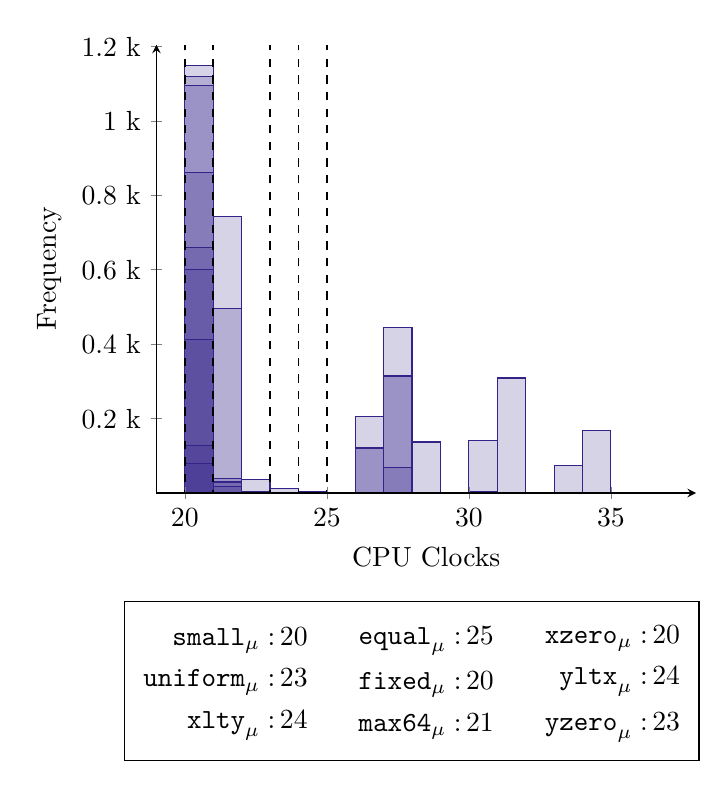
\begin{tikzpicture}[>=latex]
        \begin{axis}[
            axis x line=center,
            axis y line=center,
            name=ax,
            scaled y ticks=base 10:-3,
            ytick scale label code/.code={},
            yticklabel={\pgfmathprintnumber{\tick} k},
            xlabel={CPU Clocks},
            ylabel={Frequency},
            x label style={at={(axis description cs:0.5,-0.1)},anchor=north},
            y label style={at={(axis description cs:-0.1,.5)},rotate=90,anchor=south,yshift=4mm},
            area style,
            ymin=0,
            xmin=19,
            xmax=38,
            ymax=1205
            ]
            \addplot+ [ybar interval,mark=no,color=firstCol,fill=firstCol,fill opacity=0.2] table {
                20 78
21 496
22 35
23 1
24 0
25 0
26 1
27 0
28 0
29 0
30 141
31 309
32 0
33 0
34 1
35 0
36 1
37 1
            };
\addplot+ [ybar interval,mark=no,color=firstCol,fill=firstCol,fill opacity=0.2] table {
                20 1119
21 8
            };
\addplot+ [ybar interval,mark=no,color=firstCol,fill=firstCol,fill opacity=0.2] table {
                20 861
21 17
22 3
23 0
24 0
25 0
26 0
27 69
28 137
29 0
30 1
31 0
32 0
33 0
34 0
35 0
36 0
37 1
            };
\addplot+ [ybar interval,mark=no,color=firstCol,fill=firstCol,fill opacity=0.2] table {
                20 1148
21 10
            };
\addplot+ [ybar interval,mark=no,color=firstCol,fill=firstCol,fill opacity=0.2] table {
                20 659
21 29
22 3
23 0
24 1
25 0
26 122
27 314
28 1
29 1
30 3
31 0
32 0
33 0
34 0
35 0
36 0
37 2
            };
\addplot+ [ybar interval,mark=no,color=firstCol,fill=firstCol,fill opacity=0.2] table {
                20 413
21 39
22 1
23 0
24 3
25 0
26 205
27 445
28 2
29 1
30 0
31 0
32 0
33 0
34 0
35 1
36 0
37 1
            };
\addplot+ [ybar interval,mark=no,color=firstCol,fill=firstCol,fill opacity=0.2] table {
                20 1094
21 11
            };
\addplot+ [ybar interval,mark=no,color=firstCol,fill=firstCol,fill opacity=0.2] table {
                20 128
21 743
22 0
23 13
24 3
25 0
26 0
27 0
28 1
29 2
30 0
31 0
32 0
33 75
34 169
35 0
36 0
37 2
            };
\addplot+ [ybar interval,mark=no,color=firstCol,fill=firstCol,fill opacity=0.2] table {
                20 600
21 32
22 1
23 1
24 1
25 0
26 120
27 315
28 1
29 0
30 1
31 1
32 0
33 0
34 0
35 0
36 0
37 2
            };
                                \draw[color=black, line width=0.2mm, dashed] 
                (axis cs:25, -60.25) -- (axis cs:25, 1205);
                \draw[color=black, line width=0.2mm, dashed] 
                (axis cs:20, -60.25) -- (axis cs:20, 1205);
                \draw[color=black, line width=0.2mm, dashed] 
                (axis cs:21, -60.25) -- (axis cs:21, 1205);
                \draw[color=black, line width=0.2mm, dashed] 
                (axis cs:20, -60.25) -- (axis cs:20, 1205);
                \draw[color=black, line width=0.2mm, dashed] 
                (axis cs:23, -60.25) -- (axis cs:23, 1205);
                \draw[color=black, line width=0.2mm, dashed] 
                (axis cs:24, -60.25) -- (axis cs:24, 1205);
                \draw[color=black, line width=0.2mm, dashed] 
                (axis cs:20, -60.25) -- (axis cs:20, 1205);
                \draw[color=black, line width=0.2mm, dashed] 
                (axis cs:24, -60.25) -- (axis cs:24, 1205);
                \draw[color=black, line width=0.2mm, dashed] 
                (axis cs:23, -60.25) -- (axis cs:23, 1205);
        \end{axis} 
        \node[below=15mm of ax] (1) {
            $\begin{aligned}
                \texttt{equal}_\mu: & \,25\\
                \texttt{fixed}_\mu: & \,20\\
                \texttt{max64}_\mu: & \,21
            \end{aligned}$
        };
        \node[left=4mm of 1] (2) {
            $\begin{aligned}
                \texttt{small}_\mu: & \,20\\
                \texttt{uniform}_\mu: & \,23\\
                \texttt{xlty}_\mu: & \,24
            \end{aligned}$
        };
        \node[right=4mm of 1] (3) {
            $\begin{aligned}
                \texttt{xzero}_\mu: & \,20\\
                \texttt{yltx}_\mu: & \,24\\
                \texttt{yzero}_\mu: & \,23
            \end{aligned}$
        };
        \node[fit=(1)(2)(3),draw]{};
        \end{tikzpicture}%
      \end{lrbox}\resizebox{\textwidth}{!}{\usebox{\mybox}}
      \caption{Fuzzing results visualized. The means of each fuzz class are shown as vertical lines.}
    \end{subfigure}
    \hspace{1cm}
    \begin{subfigure}[b]{0.3\textwidth}
      \begin{lstlisting}[style=defstyle,language={[x86masm]Assembler},basicstyle=\footnotesize\ttfamily,breaklines=true]
...
  pushq	%rbp
  movq	%rsp, %rbp
  movq	%rdi, -8(%rbp)
  movq	%rsi, -16(%rbp)
  cmpq	$0, -8(%rbp)
  js	.L2
  movl	$-29, %eax
  movl	$-37, %edx
  movl	%eax, %ecx
  sarl	%cl, %edx
  movl	%edx, %eax
  cmpl	$1, %eax
  jle	.L3
.L2:
  movl	$1, %eax
  jmp	.L5
.L3:
  movl	$0, %eax
.L5:
  popq	%rbp
  ret
...\end{lstlisting} 
       \caption{Fuzzed assembly code.}
  \end{subfigure}
  \caption{An example of a true positive, i.e. a variable-time program that was rejected by Welch's t-test, from the \texttt{O0} dataset. 
  The source code of the program is shown in Appendix \ref{appendix:general-optimizations-results}. 
  Notice that inputs from the input classes \texttt{small}, \texttt{xzero}, \texttt{fixed} and \texttt{max64} are significantly faster than the rest.
  That is because the program branches on whether $x$ is signed or not (\texttt{js} instruction in line 7), which it never is in these 4 classes.}
  \label{fig:general-optimizations-O0-true-positive}
\end{figure}

Findings from the other datasets also deserve mentioning.
The \texttt{O1}, \texttt{O2}, \texttt{O3} and \texttt{Os} datasets had several false negatives, i.e. programs that were not rejected by Welch's t-test, but were variable-time.
Concretely, we saw examples where the assembled code branched on a \textit{very} specific scenario, e.g. if $x = 8129346172934691$, which is near-impossible to detect by fuzzing since the probability of hitting that specific value is very low.
We did not find any false positives in any other dataset than \texttt{O0}.
This is because the vast majority of programs in the \texttt{O1}, \texttt{O2}, \texttt{O3} and \texttt{Os} datasets were variable-time.
This points to the fact that more aggressive optimizations that introduce conditional branching are more likely to produce actual variable-time machine code.
The reason that Welch's t-test did not detect vulnerabilities in all programs in the datasets is likely due to the above-mentioned false negatives, but also because the t-test has some inherent limitations as mentioned in Section \ref{sec:statistical-analysis}.
Concrete examples of true and false positives and negatives can be found in Appendix \ref{appendix:general-optimizations-results}.

Finally, we want to address the fact that the general optimizations datasets were generated with programs that had ASTs of max depth 5.
This was done to reduce the length of the programs to make them more manageable for analysis.
However, we also generated datasets with ASTs of max depth 12 and found that the results were similar in the \texttt{O0} and \texttt{O1} datasets, while the \texttt{O2}, \texttt{O3} and \texttt{Os} datasets had significantly more programs with conditional branching -- around 5\%, 5\% and 2\% respectively.
We deem the choice of max depth 5 to be a good compromise between the length of the programs and the number of conditional branches since our results underline the problem we are trying to address.

\subsection{Specific Optimizations}
\label{sec:specific-optimizations}
The results in Table \ref{tab:general-optimizations} show that the percentage of vulnerable programs is the highest for the \texttt{O0} dataset, then it decreases significantly for the \texttt{O1} dataset, and then it increases significantly for the \texttt{O2} and \texttt{O3} datasets.
The significant decrease from \texttt{O0} to \texttt{O1} points to the fact that some optimizations in \texttt{gcc} decrease the number of conditional branches. 
Despite running several hundred experiments testing each possible configurable optimization flag \citep{gcc-manual} individually, we were not able to identify which optimizations were responsible for this decrease.
Furthermore, applying all configurable optimizations from \texttt{O1} to \texttt{O0} at once did not result in a decrease in the number of conditional branches.
This points to the fact that the responsible optimizations are non-configurable, i.e. they are always enabled for \texttt{O1}.
This also underlines the fact that all the \texttt{O*} flags enable optimizations that are non-configurable \citep{gcc-manual}, which in turn gives the developer less control over disabling problematic optimizations to increase the security of the code.

The significant increase from \texttt{O1} to \texttt{O2} and \texttt{O3} points to the fact that some optimizations in \texttt{gcc} can introduce conditional branches and therefore timing vulnerabilities. 
We identified a configurable compiler optimization that was responsible for introducing conditional branches in our datasets: \texttt{ftree-pre}.
This optimization performs partial redundancy elimination \citep{gcc-manual}.
\texttt{ftree-pre} is enabled by default for \texttt{O2}, \texttt{O3}, and \texttt{Os}, but not for \texttt{O1}.

Partial redundancy elimination (PRE) is a form of common subexpression elimination (CSE) that tries to eliminate redundant computations. 
We discussed how CSE works and how it can introduce conditional branches in Section \ref{sec:cse}.
Specifically, PRE tries to eliminate computations that are redundant in some, but not all, control flow paths.
This is done by moving the computation to a point in the program where it is guaranteed to be executed only once.
This results in different control flow paths with different amounts of instructions, which in turn result in timing vulnerabilities.

\subsection{Vulnerable Expressions}
\label{sec:vulnerable-expressions}
Finally, we identified various types of expressions that were compiled into conditional branches.
We identified expressions on the form $c$ \texttt{op} $x$ \texttt{comp} $y$, where $c$ is a constant, \texttt{op} is a bitwise operator, \texttt{comp} is a comparison operator, and $x$ and $y$ are variables.
Expressions of this form result in constant-time code containing conditional branches, much like the example in Figure \ref{fig:assembly-inspection-example}.

A more severe type of expression that we identified was expressions on the form $undefined$ \texttt{op} $(x$ \texttt{comp} $y)$, where $undefined$ contains undefined behavior, \texttt{op} is a bitwise operator, \texttt{comp} is a comparison operator, and $x$ and $y$ are variables. 
Expressions of this form sometimes result in variable-time code when compiled with \texttt{O0}.
However, when compiled with \texttt{O1}, \texttt{O2}, \texttt{O3} or \texttt{Os}, the entire program is optimized away and replaced with \texttt{return 0;}.
This is because the compiler can deduce that the expression contains undefined behavior, and, according to the C standard, the compiler is allowed to replace undefined behavior with anything \citep{c-standard}.
An example of this type of expression and its corresponding assembly, when compiled with \texttt{O0}, is shown in Figure \ref{fig:vulnerable-expression}.

\begin{figure}[H]
  \centering
     \begin{subfigure}[b]{0.41\textwidth}
        \begin{lstlisting}[style=defstyle,language={C},basicstyle=\ttfamily,breaklines=true]
int program(long long int x, long long int y) { 
  return (42 >> -1) & (x == y); 
}\end{lstlisting} 
      \vspace{6em}
      \caption{An example of a program containing an expression of the form $undefined$ \texttt{op} $(x$ \texttt{comp} $y)$.
      Specifically, bit-shifting with a negative number is undefined behavior in C \citep{c-standard}.}
    \end{subfigure}
    \hspace{1cm}
    \begin{subfigure}[b]{0.3\textwidth}
      \begin{lstlisting}[style=defstyle,language={[x86masm]Assembler},basicstyle=\footnotesize\ttfamily,breaklines=true]
...
  pushq   %rbp
  movq    %rsp, %rbp
  movq    %rdi, -8(%rbp)
  movq    %rsi, -16(%rbp)
  movq    -8(%rbp), %rax
  cmpq    -16(%rbp), %rax
  jne     .L2
  movl    $-1, %eax
  movl    $42, %edx
  movl    %eax, %ecx
  sarl    %cl, %edx
  movl    %edx, %eax
  andl    $1, %eax
  jmp     .L4
.L2:
  movl    $0, %eax
.L4:
  popq    %rbp
  ret
...\end{lstlisting} 
       \caption{Corresponding assembly code when compiled with \texttt{O0} in \texttt{gcc}.}
  \end{subfigure}
  \caption{An example of a small program that causes \texttt{gcc} to generate variable-time code when compiled with \texttt{O0}. Specifically, one can obtain whether $x$ is equal to $y$ by timing the program.}
  \label{fig:vulnerable-expression}
\end{figure}

Finally, and perhaps most importantly, we identified expressions that will result in variable-time code when compiled with \texttt{O2}, \texttt{O3} and \texttt{Os}.
As mentioned in Section \ref{sec:specific-optimizations}, partial redundancy elimination (PRE) can introduce conditional branches.
PRE is enabled for \texttt{O2}, \texttt{O3} and \texttt{Os} \citep{gcc-manual}.
In some expressions of the form $e$ \texttt{comp} $e'$, where $e$ and $e'$ contain subexpressions that are not common between $e$ and $e'$, PRE will introduce conditional branches. An example of this is shown in Figure \ref{fig:pre-example}.

\begin{figure}[H]
  \centering
  \begin{lstlisting}[style=defstyle,language={C},basicstyle=\ttfamily,breaklines=true, xleftmargin=3cm, xrightmargin=3cm]
int program(long long int x, long long int y) { 
  return 42 * (x == 42) == (y == 42); 
}\end{lstlisting} 
    \caption{An example of a program that will be variable-time when compiled with \texttt{O2}, \texttt{O3} or \texttt{Os}, specifically because of PRE.
    PRE will identify two control flow paths in this expression: 
    One where $x=42$ and one where $x \neq 42$.
    If $x=42$, the expression will always evaluate to $0$ since \texttt{42 * (42 == 42) == (y == 42)} will evaluate to $42 \stackrel{?}{=} 0$ or $42 \stackrel{?}{=} 1$ which is false in both cases.
    If $x \neq 42$, the expression depends on whether $y=42$.
    Hence \texttt{(y == 42)} is redundant in the first control flow path, but not in the second.
    As a result, PRE will insert a conditional branch that branches on $x = 42$ and only considers $y$ if that is \textit{not} the case.}
    \label{fig:pre-example}
\end{figure}


\section{Evaluation}
\todo{Evaluation of OptiFuzz and analysis. Is it accurate?}

\todo{From results, we can see that most programs with conditional branches are rejected by the t-test.
This means that our underapproximation by the inspection is okay.}

\section{Discussion}
From the previous sections, it is clear that modern compilers introduce timing vulnerabilities in constant-time programs.
This is devastating for security since it means that developers cannot reliably write constant-time code.
A solution is required.
In this section, we discuss how the problem can be solved and what the implications different solutions have on security and efficiency.

As shown in Section \ref{sec:gcc-vs-clang}, \texttt{clang} is much more conservative when it comes to inserting conditional branches in constant-time programs.
Instead of inserting variable-time conditional branches, \texttt{clang} uses constant-time conditional moves to implement branching control flow.
From this observation, it might be tempting to conclude that always substituting conditional branches with conditional moves is the solution to the problem.
However, there is more to the story.

\texttt{cmov} instructions severely restrict the out-of-order engine on modern CPUs since \texttt{cmov} instructions increase the data dependency between instructions significantly \citep{intel-optimization-reference}. 
Furthermore, branch predictions are not used for \texttt{cmov} instructions, which can lead to significant performance degradation.
Hence, we have to address this trade-off between security and efficiency.

\subsection{Forcing \texttt{cmov} Instructions When Necessary}
This trade-off between security and efficiency has led multiple researchers to propose solutions that only force \texttt{cmov} instructions to be used on critical data \citep{what-you-c,llvm-issues-blog-post}.
In both studies, the authors propose to add the possibility to specify forced \texttt{cmov} instructions in the source code and restrict the backend of the compiler to not being able to optimize the \texttt{cmov} away for those specific instructions.
This solution has the advantage that it does not affect the performance of non-critical parts of the program.
In fact, \citeauthor{what-you-c} show that their solution only introduces a performance penalty of 1\% and sometimes even increases performance.

However, this solution also has its disadvantages.
First, the solution relies heavily on the developer.
The developer has to know which parts of the program are critical, and also be able to use the language extension correctly.
In turn, it means that security relies on human factors, which are error-prone.
Second, the solution relies on the compiler being configurable to avoid forced \texttt{cmov} instructions being optimized away.
As we discussed in Section \ref{sec:gcc-vs-clang} and \ref{sec:general-optimizations}, \texttt{clang} seems to be quite configurable while \texttt{gcc} does not.
Hence, the solution might not be easily applicable to all compilers.

Another solution is to implement vulnerable parts of the program using a domain-specific language that is designed to be constant-time.
\citeauthor{fact} proposed a domain-specific language, called FaCT, for implementing constant-time cryptographic algorithms \citep{fact}.
FaCT is designed to be interoperable with C, and the compiler ensures constant-time code by leveraging the \texttt{ct-verif} tool that is based on verification of the LLVM IR \cite{verifying-constant-time-llvm}.
\texttt{ct-verif} operates on a formalization of constant-time code and verifies based on a theoretically sound and complete methodology.
However, \citeauthor{verifying-constant-time-llvm} note that the verification process of \texttt{ct-verif} is not guaranteed to identify all timing vulnerabilities due to translation between the LLVM IR and machine code, and due to possible incompleteness of their formalization of constant-time code. 
Some of these issues were experimentally verified.
However, generally \texttt{ct-verif} captures significantly more timing vulnerabilities than other verification alternatives \citep{verifying-constant-time-llvm}.
Additionally, \texttt{ct-verif} is efficient at verifying constant-time code, often being much faster than the compilation step, but occasionally being a few times slower.

\subsection{Bullet-proofing the Compiler}
A more radical approach is to force the compiler to always produce constant-time code.
\citeauthor{verified-constant-time-c-comiler} provides a formally verified constant-time C compiler, built on top of the CompCert verified C compiler \citep{verified-constant-time-c-comiler}. 
The constant-time CompCert compiler guarantees that constant-time source code is compiled into constant-time machine code.
This is achieved by instrumenting the operational semantics of CompCert's IR to be able to capture cryptographic constant-time and proving that cryptographic constant-time is preserved during compilation. 
This has immense advantages for security.

However, the security advantages come at the cost of efficiency. 
The constant-time CompCert compiler is significantly slower than \texttt{gcc}.
Experimental results show an efficiency penalty of well over 100\% in some cases \citep{verified-constant-time-c-comiler}.

\subsection{Testing Solutions}
The final category of solutions we identified is black-box testing solutions like DudeCT \citep{dudect} and our tool OptiFuzz.
Concretely, one can test specific implementations for timing vulnerabilities using these tools.
These tests can even be automated to run as part of a continuous integration pipeline.
Solutions in this category have the obvious advantage that they are simple and require no modeling of hardware behavior or language semantics.
It is arguably the most practical solution since it does not require any changes to the compiler or the language.
It also does not induce any performance penalty.

The testing solutions, however, come with a significant security disadvantage in that they are noisy and not exact.
As we showed in Section \ref{sec:general-optimizations}, OptiFuzz will produce false positives and false negatives.
\citeauthor{dudect} raised similar concerns for DudeCT.
Fuzzing tools provide more of an indication of the presence of timing vulnerabilities than a guarantee.

\todo{Argue that many solutions exist with a mixture of security and efficiency.
We argue that people should start using them.
Perhaps OptiFuzz + compromise solutions}

\section{Conclusion and Future Work}
We have a lot of ideas for future work that we did not get around to. These include:
\begin{itemize}
    \setlength\itemsep{-0.6em}
    \item Extend OptiFuzz to generate more complicated programs, eg. by reintroducing the division and modulus operators while dealing with division by zero in a meaningful way.
    \item Increasing the precision of the assembly inspection. One way could be to detect if branches contain the same amount of work and identify them as constant time.
    \item Implement other relevant input classes. A dynamic class containing the hardcoded values from a program. This might be able to catch the very specific but unpredictable values that courses branching.
    \item Extending the usage of Welsh's t-test to all classes, and not just between \texttt{uniform} and \texttt{fixed}.
    \item Create a tool that warns developers in real-time about constant C expressions that might be compiled to variable time by comparing it to a database precomputed using OptiFuzz. This tool could furthermore be implemented in a CI/CD environment.
    \item Extend OptiFuzz to support other processor architecture, especially including ones used by embedded systems.
\end{itemize}


\pagebreak

\bibliographystyle{abbrvnat}
\bibliography{litterature}

\pagebreak
\begin{appendices}

\section{Select General Optimizations Results}
\label{appendix:general-optimizations-results}
%\documentclass[10pt]{article}
\usepackage[left=0.8in,right=0.8in,bottom=0.5in,top=0.5in]{geometry}
\geometry{a4paper}
\usepackage[parfill]{parskip}    % Activate to begin paragraphs with an empty line rather than an indent
\usepackage{graphicx}
\usepackage{xcolor}
\usepackage{hyperref}
\usepackage{titling}
\usepackage[small,compact]{titlesec}
\usepackage[toc,page]{appendix}

\usepackage{listings}
\usepackage{pgfplots}
\usepackage{adjustbox}
\usepackage{float}
\usepackage{subcaption}
\usepackage{pgffor}
\usepackage{expl3}
\usepackage{xparse}
\usepackage{xfp}
\usetikzlibrary{fit}
\usetikzlibrary{positioning}


\usepackage{amsmath,amssymb}
\DeclareGraphicsRule{.tif}{png}{.png}{`convert #1 `dirname #1`/`basename #1 .tif`.png}



\newcommand\courseName{Language-Based Security}
\newcommand\courseNameAbbrv{LBS}
\newcommand\courseYear{2023}
\newcommand\courseAndYear{\courseNameAbbrv-\courseYear}
\newcommand\reportKind{Exam Report}

\newcommand\groupNumber[1]{
  \makeatletter
  \def\@courseGroupNumber{#1}
  \makeatother
}

\pretitle{\begin{flushright} \bfseries  \large \courseAndYear: \reportKind \end{flushright}   \begin{flushleft}
\bfseries \LARGE}
\posttitle{\par\end{flushleft}\vskip 0.5em}

\preauthor{
\begin{flushleft}
\large \lineskip 0.5em%
\bfseries
\makeatletter Group \@courseGroupNumber \\ \makeatother
\begin{tabular}[t]{@{}l}}
\postauthor{\end{tabular}\par\end{flushleft}}

\predate{\begin{flushleft}\bfseries \large}
\postdate{\par\end{flushleft}}

\usepackage{listings}
\usepackage{pgfplots}
\usepackage{adjustbox}
\usepackage{float}
\usepackage{subcaption}
\usepackage{pgffor}
\usepackage{expl3}
\usepackage{xparse}
\usepackage{xfp}

\newcommand\todo[1]{\textcolor{red}{TODO: #1}}

\pgfplotsset{compat=1.12}

\definecolor{mGreen}{rgb}{0,0.6,0}
\definecolor{mGray}{rgb}{0.5,0.5,0.5}
\definecolor{mPurple}{rgb}{0.58,0,0.82}
\definecolor{backgroundColour}{rgb}{0.95,0.95,0.92}

\definecolor{firstCol}{HTML}{332288}
\definecolor{secondCol}{HTML}{117733}
\definecolor{thirdCol}{HTML}{44AA99}
\definecolor{fourthCol}{HTML}{88CCEE}
\definecolor{fifthCol}{HTML}{DDCC77}
\definecolor{sixthCol}{HTML}{DD2255}

\lstdefinestyle{defstyle}{
    backgroundcolor=\color{backgroundColour},   
    commentstyle=\color{mGreen},
    keywordstyle=\color{magenta},
    numberstyle=\tiny\color{mGray},
    stringstyle=\color{mPurple},
    basicstyle=\footnotesize,
    breakatwhitespace=false,         
    breaklines=true,                 
    captionpos=b,                    
    keepspaces=true,                 
    numbers=left,                    
    numbersep=5pt,                  
    showspaces=false,                
    showstringspaces=false,
    showtabs=false,                  
    tabsize=2
}

\newsavebox{\mybox}

\ExplSyntaxOn
\cs_new:Npn \__afp_ismember_loop:Nnw #1#2#3,
  {
    \quark_if_recursion_tail_stop_do:nn {#3}
      { \prg_return_false: }
    #1 {#2} {#3}
      { \use_i_delimit_by_q_recursion_stop:nw { \prg_return_true: } }
      { \__afp_ismember_loop:Nnw #1 {#2} }
  }
\prg_new_conditional:Npnn \afp_int_ismember:nn #1#2 { p, T, F, TF }
  {
    \__afp_ismember_loop:Nnw \__afp_int_isequal:nnTF {#1} #2 ,
    \q_recursion_tail , \q_recursion_stop
  }
\prg_new_conditional:Npnn \__afp_int_isequal:nn #1#2 { p, T, F, TF }
  {
    \int_compare:nNnTF {#1} = {#2}
      { \prg_return_true: }
      { \prg_return_false: }
  }
\NewExpandableDocumentCommand { \IncludeExperimentResults } { m m }
  {
    \foreach \x in {1,...,#1} {
        \noindent\bool_if:NF { \afp_int_ismember_p:nn {\x} {#2} } {\input{generated_latex/prog\x.tex}}
    }
  }
\ExplSyntaxOff
\usepackage[authoryear]{natbib}

\title{
  Optimizing Away Security in C
}

\groupNumber{10}
\author{Anders B. Clausen \and Johan T. Degn \and Jonathan Eilath}

\begin{document}
\maketitle
\thispagestyle{empty}

\section*{Abstract}
\todo{After the paper is done}

\section{Introduction}
The C programming language is one of the most widely used programming languages in the world. 
It is used in a wide variety of applications, ranging from embedded systems to cryptographic libraries. 
However, C is also notorious for lacking security guarantees.
Security-related issues in programs written in C stem from both the programmer, but also from the compiler.

The problem with security issues introduced by the compiler is especially prevalent in the context of timing attacks on cryptographic algorithms. 
Developers try to mitigate timing attacks by writing constant-time code -- code where the execution time is independent of the input.
However, the compiler may introduce timing leaks by optimizing away the constant-time code.
In a recent study \citep{developer-survey-timing-attacks}, it was shown that the vast majority of developers of cryptographic libraries rely on constant-time code practices that in theory result in constant-time code, but may be vulnerable after compilation.

The issue of timing vulnerabilities introduced by compilers is well-known in the community.
Several proposals have been made to mitigate the issue \citep{what-you-c, dudect, fact, verified-constant-time-c-comiler}.
However, the problem persists and to the best of our knowledge, no study has quantified the issue of timing vulnerabilities introduced by compilers.

In this paper, we try to quantify the issue of timing vulnerabilities introduced by the two most popular C compilers, gcc\footnote{\url{https://gcc.gnu.org/}.} and clang\footnote{\url{https://clang.llvm.org/}.}.
We do this by implementing a tool, OptiFuzz, that generates, analyzes and fuzzes random C programs.
For simplicity, the generated programs are limited to only containing non-branching arithmetic, logical and comparison operations.
Also \texttt{/} and \texttt{\%} are avoided, to mitigate division-by-zero errors.
We investigate what optimization flags are responsible for introducing timing leaks and compare them.
Finally, we discuss how the issue of timing vulnerabilities introduced by the compiler can be mitigated by using language-based security techniques.

\subsection{Related Work}
The issue of timing vulnerabilities introduced by the clang C compiler across different versions has been researched by Simon et. al. \citep{what-you-c}. 
Several studies have investigated potential solutions to the issue, including using constant-time branching instructions \citep{what-you-c}, using black-box testing software \citep{dudect}, domain-specific languages \citep{fact}, and notably a verified constant-time C compiler has been developed \citep{verified-constant-time-c-comiler}.

\subsection{Contributions}
We provide a quantitative analysis of timing vulnerabilities introduced by gcc and clang, focusing on specific troublesome optimization flags.
Additionally, we provide a tool, OptiFuzz, that can be used to generate, analyze and fuzz random C programs for further investigation of the issue.
\todo{Might be more when we finish the paper}
\subsection{Overview}
This paper is organized as follows: $\ldots$ 
\todo{After we have finished the rest of the paper}
\todo{Insert guide on how to read appendix here??}

\section{Preliminaries}
\subsection{Timing Attacks}
Timing attacks are a class of side-channel attacks that exploit the fact that the execution time of a program can depend on the input.
The history of timing attacks goes back several decades where Kocher showed multiple successful timing attacks on well-known cryptographic algorithms such as Diffie-Hellman and RSA \citep{1996-timing-attacks}.
An example of vulnerable code is shown in Figure \ref{fig:timing-attack-example}.
\begin{figure}[H]
  \begin{lstlisting}[style=defstyle,language=C, xleftmargin=6.8cm, xrightmargin=6.8cm]
int foo(int x) {
  if (x < 100) {
    x *= 2;
    x += 7;
  }
  return x;
} \end{lstlisting} 
  \caption{Example of a program vulnerable to a timing attack. 
  Only by analyzing the execution time of the machine code, an attacker can infer whether the input is less than 100 or not.}
  \label{fig:timing-attack-example}
\end{figure}

\subsection{Optimizing Compilers}
Cryptographers will avoid code like the example in Figure \ref{fig:timing-attack-example} and write constant-time code instead.
Constant-time code is code where the execution time is independent of the input.
However, the compiler may introduce timing vulnerabilities through optimizations by adding variable-time branches to the machine code.
The issue arises in the analysis and transformation phases of the compiler as illustrated in Figure \ref{fig:optimizing-compiler-pipeline}.

\begin{figure}[H]
  \centering
  \tikzstyle{box} = [rectangle, minimum width=2.8cm, minimum height=1cm, text centered, draw=black]
\tikzstyle{arrow} = [thick,->,>=stealth]

\begin{tikzpicture}
  \node (Source Code) [box] {Source Code};
  \node (Lexing) [box, fill=lightgray, right of=Source Code, xshift=2.5cm] {Lexing};
  \node (Parsing) [box, fill=lightgray, right of=Lexing, xshift=2.5cm] {Parsing};
  \node (AST) [box, right of = Parsing, xshift=2.5cm] {AST};
  \node (Semantic Analysis) [box, fill=lightgray, right of=AST, xshift=2.5cm] {Semantic Analysis};
  \node (Intermediate Representation) [box, below of=Semantic Analysis, yshift=-1.2cm, xshift=0cm] {IR};
  \node (Analysis) [box, fill=lightgray, left of=Intermediate Representation, xshift=-2.5cm] {Analysis};
  \node (Transformation) [box, fill=lightgray, left of=Analysis, xshift=-2.5cm] {Transformation};
  \node (Code Generation) [box, fill=lightgray, left of=Transformation, xshift=-2.5cm] {Code Generation};
  \node (Executable) [box, left of=Code Generation, xshift=-2.5cm] {Executable};

  \draw [arrow] (Source Code) -- (Lexing);
  \draw [arrow] (Lexing) -- (Parsing);
  \draw [arrow] (Parsing) -- node [fill=white, text=darkgray, yshift=0.9cm] {Syntactically Sound} (AST);
  \draw [arrow] (AST) -- (Semantic Analysis);
  \draw [arrow] (Semantic Analysis) -- node [fill=white, text=darkgray] {Semantically Sound} (Intermediate Representation);
  \draw [arrow] (Intermediate Representation) -- (Analysis);
  \draw [arrow] (Analysis) -- (Transformation);
  \draw [arrow, dashed] (Transformation) to [bend left=25] (Intermediate Representation);
  \draw [arrow] (Transformation) -- node [fill=white, text=red, yshift=0.9cm] {Optimized} (Code Generation);
  \draw [arrow] (Code Generation) -- (Executable);
\end{tikzpicture}
  \caption{The pipeline of an optimizing compiler. After the transformation phase, the IR is optimized and the compiler may have introduced timing vulnerabilities.}
  \label{fig:optimizing-compiler-pipeline}
\end{figure}

Many different kinds of optimization techniques are carried out by optimizing compilers, some of which can introduce timing vulnerabilities.
Some common optimization techniques like common subexpression elimination and strength reduction have been shown to introduce timing vulnerabilities \citep{optimizations-linked-to-timing-attacks}.
To illustrate this point, we look at how common subexpression elimination can introduce timing vulnerabilities.

\subsubsection{Timing Vulnerabilities Through Common Subexpression Elimination}
Common Subexpression Elimination is an optimization technique that extracts subexpressions that are common across multiple expressions and replaces them with a single variable.
This optimization technique can introduce timing vulnerabilities since it can decrease the number of instructions executed for a specific branch of the code as illustrated in Figure \ref{fig:common-subexpression-elimination}.
Here the common subexpression \texttt{2 * 3 + 5} is extracted and assigned to the variable \texttt{common}, making the \texttt{else} branch execute faster than the \texttt{if} branch.

\begin{figure}[H]
  \centering
     \begin{subfigure}[b]{0.3\textwidth}
        \begin{lstlisting}[style=defstyle, language=C]
int foo(int x, int *arr) {
  if (x == SECRET) {
    x = arr[0] * 3 + 5;
    x += arr[1] * 3 + 5;
    x += arr[2] * 3 + 5;
  } else {
    x = 2 * 3 + 5;
    x += 2 * 3 + 5;
    x += 2 * 3 + 5;
  }
  return x;
} \end{lstlisting} 
         \caption{Original code.}
    \end{subfigure}
    \hspace{1cm}
    \begin{subfigure}[b]{0.3\textwidth}
      \begin{lstlisting}[style=defstyle, language=C]
int foo(int x, int *arr) {
  if (x == SECRET) {
    x = arr[0] * 3 + 5;
    x += arr[1] * 3 + 5;
    x += arr[2] * 3 + 5;
  } else {
    // optimized
    int common = 2 * 3 + 5;
    x = 3 * common;
  }
  return x;
} \end{lstlisting} 
       \caption{Optimized code.}
  \end{subfigure}
  \caption{An example of how the common subexpression elimination can introduce timing vulnerabilities in code. (a) shows the original code and (b) shows the optimized code.}
  \label{fig:common-subexpression-elimination}
\end{figure}

\section{OptiFuzz}
We created a tool, OptiFuzz, that can be used to generate, analyze and fuzz random C programs.
The source code for OptiFuzz is available on GitHub\footnote{\url{https://github.com/anbclausen/optifuzz}.}.
The goal of OptiFuzz is to quantify the issue of timing attacks introduced by C compilers with different optimization flags enabled.
The tool works as follows:
\begin{itemize}
  \item OptiFuzz generates random C programs consisting of non-branching arithmetic, logical and comparison operations.
  \item OptiFuzz then compiles the generated C programs with different specified optimization flags enabled and inspects the generated assembly for branching instructions introduced by the compiler.
        If branching is found, the program is flagged.
  \item OptiFuzz then fuzzes the flagged programs with various random inputs to test whether the branching instructions can be exploited to leak information about the input.
  \item At last, OptiFuzz reports the results of the fuzzing in the form of a PDF report.
\end{itemize}
The OptiFuzz pipeline is illustrated in Figure \ref{fig:optifuzz-pipeline}. 
Each of the steps in the pipeline is described in detail in the following sections.
\begin{figure}[H]
  \centering
  \tikzstyle{box} = [rectangle, minimum width=3cm, minimum height=1cm, text centered, draw=black]
\tikzstyle{arrow} = [thick,->,>=stealth]

\begin{tikzpicture}
  \node (Code Generation) [box] {Code Generation};
  \node (Assembly Inspection) [box, right of=Code Generation, xshift=3cm] {Assembly Inspection};
  \node (Fuzzing) [box, right of=Assembly Inspection, xshift=3cm] {Fuzzing};
  \node (Visualization) [box, right of=Fuzzing, xshift=3cm] {Visualization};

  \draw [arrow] (Code Generation) -- (Assembly Inspection);
  \draw [arrow] (Assembly Inspection) -- (Fuzzing);
  \draw [arrow] (Fuzzing) -- (Visualization);
\end{tikzpicture}
  \caption{The OptiFuzz pipeline.}
  \label{fig:optifuzz-pipeline}
\end{figure}




\subsection{Code Generation}
The first step in the OptiFuzz pipeline is code generation. 
The code generation module is written in OCaml and works by generating abstract syntax trees according to the grammar in Figure \ref{fig:grammar}.

\begin{figure}[H]
  \centering
  \begin{align*}
    e \in Expr ::= & x \mid y &\text{(input variables)}\\
    & n \in \{0, 1\}^{64} &\text{(64-bit integer literals)}\\
    & -e \mid e + e \mid e - e \mid e \times e &\text{(arithmetic operators)}\\
    & \texttt{true} \mid \texttt{false} &\text{(boolean literals)}\\
    & !e &\text{(logical operators)}\\
    & e < e \mid e \leq e \mid e > e \mid e \geq e \mid e = e \mid e \neq e &\text{(comparison operators)}\\
    & e \texttt{\&} e \mid e \texttt{|} e \mid \text{\~{}} e \mid e \text{\^{}} e \mid e \ll e \mid e \gg e &\text{(bitwise operators)}
  \end{align*}
  \caption{The grammar that defines the ASTs generated by the code generation module in the OptiFuzz pipeline.}
  \label{fig:grammar}
\end{figure}

The grammar defines all programs with 2 variables and non-branching arithmetic, logical and comparison operations in C \citep{c-standard}, excluding division (\texttt{/}) and modulus (\texttt{\%}).
The reason for excluding division and modulus is that they may cause division-by-zero errors.
Generated programs are forced to include both input variables, $x$ and $y$.
$x$ and $y$ are the inputs to the program, and we require both to be present since programs with 0 or 1 input variables are trivially constant-time.
An example of a program generated by the code generation module is shown in Figure \ref{fig:code-gen-example}.

\begin{figure}[H]
  \begin{lstlisting}[style=defstyle,language=C, xleftmargin=2.7cm, xrightmargin=2.7cm]
#define false 0
#define true 1
int program(int x, int y) { return !(y * (43 * (x != true))); } \end{lstlisting}
  \caption{Example of a program generated by the code generation module.}
  \label{fig:code-gen-example}
\end{figure}

The code generation module works by generating a random distribution that selects different symbols in the grammar with a certain probability.
This ensures that not all generated programs will be uniformly random.
For example, if a generated distribution heavily favors the left-shift operator, then the generated programs will contain a lot of left-shift operations.
This is useful for detecting whether certain types of programs are more likely to be constant-time than others.

The code generation module generates programs with integer literals in different ranges. 
Booleans represent the first range.
Defining Booleans as integers is a common practice in C \citep{c-standard}.
Integers from this range are included since the constants 0 and 1 are interesting in many operations.
The second range we consider is $[0, 64]$ as numbers in this range are lower than the size of 64-bit integers.
Hence numbers in this range are interesting in bit-shifting operations.
The third range is the range of signed 64-bit integers.
Generally, we have included these smaller ranges of integers since they are interesting and it is very unlikely that a uniformly random 64-bit integer would be in these ranges.

The grammar in Figure \ref{fig:grammar} generates programs with undefined behavior.
For example, bit-shifting with a negative number, or a number larger than the size of the type, is undefined behavior in C \citep{c-standard}.
We chose to include undefined behavior in the grammar since it is a source of timing vulnerabilities \citep{what-you-c}, and it is common in real-life code \citep{undefined-behavior-c}.
The grammar also does not distinguish operations on Booleans and integers and hence generates untypical C programs.
For example, the program in Figure \ref{fig:code-gen-example} features multiplication between a Boolean and an integer.
We chose to include this in the grammar since it is a used trick to avoid branching in constant-time code \citep{what-you-c}.

\subsubsection{Limitations}
The biggest limitation of this approach is that the generated programs are not representative of real-life code since they use such a limited subset of the C language.
However, as argued above the simple constant-time programs are representative of how real code might look, and thus gives a useful insight into the issue of timing vulnerabilities introduced by the compiler.
\subsection{Assembly Inspection}
\label{sec:inspection}

The next step in the OptiFuzz pipeline is assembly inspection.
The assembly inspection module is written in Python and works by inspecting the assembly generated by the compiler across different optimization flags.
The compiled assembly is inspected for conditional branching instructions and flagged if that is the case.
The assembly inspection module is only able to analyze x86-64 assembly.

In x86-64 assembly, \texttt{Jcc} (note, this does not include \texttt{JMP}), \texttt{LOOP} and \texttt{LOOPcc} are the only conditional branching instructions \citep{intel-reference}.
This means that the assembly inspection module only needs to look for these instructions.
Both \texttt{Jcc} and \texttt{LOOPcc} refer to a family of instructions where \texttt{cc} is a condition code.
For example, \texttt{JE} (jump if equal) is in the \texttt{Jcc} instruction family. 
We did not include conditional move instructions in the analysis since they are constant-time \citep{cmov-is-constant-time}.

\subsubsection{Limitations}
An obvious limitation of this approach is that it is tailored for x86-64 assembly.
Hence our analysis will not work for other architectures.
Furthermore, the programs that are flagged by the assembly inspection module are not necessarily vulnerable to timing attacks.
Hence, the assembly inspection module overapproximates the set of programs that are vulnerable to timing attacks.
For example, the program in Figure \ref{fig:assembly-inspection-example} is flagged by the assembly inspection module, but it is constant-time since both branches take the same amount of time to execute.

\begin{figure}[H]
  \centering
  \begin{lstlisting}[style=defstyle, language={[x86masm]Assembler}, basicstyle=\footnotesize\ttfamily,breaklines=true, xleftmargin=4cm, xrightmargin=4cm]
...
  cmpl    $1, -4(%rbp) ; compare TOS to 1
  je      .L2          ; jump to .L2 if equal
  movl    $43, %eax    ; move 43 into %eax
  jmp     .L3
.L2:
  movl    $0, %eax     ; move 0 into %eax
.L3:
  ret\end{lstlisting}
  \caption{Example of a program that is flagged by the assembly inspection module, but is constant-time.}
  \label{fig:assembly-inspection-example}
\end{figure}
\subsection{Fuzzing}
After the assembly inspection has performed the static analysis and flagged programs with potential timing vulnerabilities, the next step is to run a dynamic analysis on them to try and confirm their presence. For this, we have created a fuzzer that runs the programs compiled with the specified compiler and optimization levels fuzzing the arguments the program takes as inputs and measuring its execution time. 

The process goes as follows. First, the fuzzer itself is compiled into object files which are not yet linked. This compilation only needs to happen once. Each of the programs flagged by the static assembly analysis is then compiled one at a time with the specified compiler for each of the supplied optimization flags and linked with the pre-compiled fuzzer. This includes the flags for which the assembly inspector did not detect any branches. This creates a complete fuzzer including the program to fuzz.

The fuzzer generates inputs according to fuzzing classes. For each input it chooses a uniformly random class among the supplied ones. This way there is no biased order in which the inputs from different classes are used, and thus potential noise is likely to effect all classes equally. This is important when comparing timing distributions in the following analysis. After generating the inputs it runs through them and calls the internally linked program with each of them. The programs' execution time is measured every time it is run. The fuzzer repeats the run-through multiple times (50) to allow for detection of outliers and get as precise results as possible. Note that an input is only repeated after each of the others and not multiple times in a row. In addition to having a random class input order, this ensures that any noise that results in longer execution times are not concentrated on a few inputs but distributed over all (or many) of them. This way we minimize the chance of falsely identifying an input or class of inputs as the course of a longer execution time.

As mentioned we use different classes for the inputs to the fuzzer, instead of always generating completely random numbers. This is done to try and capture variable execution time that only takes place a small sample of the values. This could as an example be if there is a check for if one of the inputs are zero. If we only used uniformly random 64-bit numbers it would be unlikely to observe it happen. Even if it did, it would probably just be filtered out as an outlier. Hence, the need for fuzzing classes. For each input there are an $x$ and a $y$ value. The classes the following generates inputs with respect to $x$ and $y$ as seen in the following list.
\begin{itemize}
    \item UNIFORM: They are uniformly random 64-bit numbers.
    \item EQUAL:   They have the same uniformly random 64-bit number.
    \item MAX64:   A random one is a random 64-bit number, the other is uniformly random.
    \item XZERO:   $x$ is 0, $y$ is a uniformly random number.
    \item YZERO:   $y$ is 0, $x$ is a uniformly random number.
    \item XLTY:    Two uniformly random numbers are generated, $x$ is set to the smaller, $y$ to the larger.
    \item YLTX:    Two uniformly random numbers are generated, $y$ is set to the smaller, $x$ to the larger.
    \item SMALL:   They are uniformly random 8-bit numbers (the upper 56 bits are set to 0).
    \item FIXED:   They have the same fixed number $0x12345678$ (used for the T-test).
\end{itemize}
These classes have been made based on observations of values commonly used in comparison in the assembly.

Precise measurements of a program's execution time is not trivial. It can be influenced by a number of things including context switches, interrupts, out-of-order execution, varying CPU clock speed and congestion. Furthermore, since we are dealing with quite small programs that are quick to run, our options for timing them are reduced. The most obvious way to time a program is using the system clock. But when testing it, it became clear that its resolution was too low. We ended up using the Time Stamp Counter (TSC) which is a high resolution counter that (on newer machines) increase at a fixed rate independent of processor frequency. This method is heavily inspired by the suggestions and results from an Intel white paper \citep{intel-benchmark-code-execution}.
Using the TSC as a reference for time is the best we can do on our x86-64 architecture machine.
This approach also allowed us to avoid the timings being skewed by the CPU performing out-of-order execution. Out-of-order could lead to the instructions being reordered resulting in not reading the TSC (with the RDTSC(P) instruction) at the exact time we want to. This is done by utilizing the non-privileged CPUID instructions serializing capabilities that ensure that memory transactions for previous instructions are completed before the next instruction is executed \citep[a]{intel-reference}.

When later using these results in the analysis, we use the minimum time for all executions with the same input. Using the minimum time as the true execution time instead of the mean filters out the noise from outliers that are the results of i.e. context-switches or congestion, as argued in \citep{robust-benchmarking}. In comparison to the DudeCT black-box testing program from \citep{dudect}, which just removes top 5\% of the longest measured execution times to reduce such noise, our approach is not prone to accidentally removing measurements of large execution times that are correct and not the result of noise.

\subsubsection{Limitations}
As mentioned in the assembly inspection section, the inspector over approximates and might flag programs which are in fact constant time. Furthermore, we run the fuzzer for all flags if just one of them was flagged by the inspector.
Considering this, we consider the fuzzer successful when it is able to consistently measure clear differences in execution time of a program with respect to its inputs. Such time difference makes it possible to make an educated guess on what the given inputs look like, and hence opens up for a potential timing based side channel attack. This does indeed indicate that the program is vulnerable.

If, on the other hand, the results of this analysis fails to indicate obvious timing differences, then it is not safe to assume that it is then constant time. This of course could be the case since the assembly inspection over approximates. Since fuzzer is conservative and under approximates, it could be that the input classes used in fuzzing where not able to capture the event coursing the variable time. Considering it could also be constant time, we have to settle with not knowing for sure.

Even with the actions taken to get as precise timings as possible the analysis is still prone to some noise. Specifically, it is worth noting that when running this in userland the fuzzer could be influenzed by interupts and preemtion. Both of these requires the code to run in kernel space to disable, which is a possible future extension of the fuzzer. As a compromise making it this less of a source of noise the fuzzer can be run with higher priority, as is the case for our results. 

\subsection{Statistical Analysis}
\label{sec:statistical-analysis}
At the end of the pipeline, we have at our disposal flagged C programs, which have been fuzzed and timed. Now we have to conclude whether or not these programs are variable-time or not. This is a very complex task, as a lot of factors can affect this. Notably, the research conducted by \citeauthor{Abel19a} demonstrates the difficulty of this, as determining the performance of instructions is very microarchitecture dependant. Additionally, \cite{verifying-constant-time-llvm}'s work suggests that static analysis on LLVM can be done, but again suffers from architecture-specific modeling. Thus, we determined that our method should not consider all the intricate details of architecture-specific implementations. Instead, a statistical approach was deemed more suitable.

One statistical approach is to apply significance tests between classes of fuzzing inputs. If we can detect a difference in time between different kinds of inputs, then we can conclude with good probability, that the program is not constant-time. Ideally, for constant-time programs, we would expect a univariate Gaussian with low variation when we measure the running time of the program for all kinds of inputs. Likewise, ideally, for variable-time programs, we hope to see a mixture distribution composed of two (or more) Gaussians with different means. For instance, if we observe two means: $\mu_1 \neq \mu_2$, then we can conclude with good probability, that most likely a branching instruction on the input dictates whether or not the program will have a running time close to $\mu_1$ or $\mu_2$.

\pgfmathdeclarefunction{gauss}{2}{%
  \pgfmathparse{1/(#2*sqrt(2*pi))*exp(-((x-#1)^2)/(2*#2^2))}%
}

% Solution to when the first gaussian is eq to second gaussian plotted in subfigure b)
\def\gausssolution{5.170045172}
\begin{figure}[H]
\captionsetup[subfigure]{justification=centering}
\begin{subfigure}[t]{0.50\textwidth}
\resizebox{\linewidth}{!}{
    \begin{tikzpicture}
    \begin{axis}[
      no markers, domain=0:10, samples=100,
      axis lines*=left, xlabel=Clock Cycles, ylabel=Frequency,
      every axis y label/.style={at=(current axis.above origin),anchor=south},
      every axis x label/.style={at=(current axis.right of origin),anchor=west, yshift=-8mm, xshift=-20mm},
      height=5cm, width=12cm,
      xtick={1,...,10}, ytick={1,...,10},
      enlargelimits=false, clip=false, axis on top,
      ]
      \addplot [very thick,cyan!50!black] {gauss(4,1)};
      \draw[color=black, line width=0.2mm, dashed] 
      (axis cs:4, 0) -- (axis cs:4, 0.4);
    \end{axis}
\end{tikzpicture}%
}%
\caption{A constant-time program yielding\\a univariate Gaussian with $\mu = 4$.}
\label{fig:univargauss}
\end{subfigure}
\begin{subfigure}[t]{0.50\textwidth}
\resizebox{\linewidth}{!}{
    \begin{tikzpicture}
    \begin{axis}[
      no markers, domain=0:10, samples=2000,
      axis lines*=left, xlabel=Clock Cycles, ylabel=Frequency,
      every axis y label/.style={at=(current axis.above origin),anchor=south},
      every axis x label/.style={at=(current axis.right of origin),anchor=west, yshift=-8mm, xshift=-20mm},
      height=5cm, width=12cm,
      xtick={1,...,10}, ytick={1,...,10},
      enlargelimits=false, clip=false, axis on top,
      ]
      \addplot [very thick,cyan!50!black, restrict x to domain = 0:\gausssolution] {gauss(4,1)};
      \draw[color=black, line width=0.2mm, dashed] 
      (axis cs:4, 0) -- (axis cs:4, 0.4);

      \addplot [very thick,cyan!50!black, restrict x to domain = \gausssolution:10] {gauss(6,0.5)};
      \draw[color=black, line width=0.2mm, dashed] 
      (axis cs:6, 0) -- (axis cs:6, 0.8);
    \end{axis}
\end{tikzpicture}%
}%
\caption{A variable-time program, yielding a mixture\\distribution composed of two Gaussian distributions\\having means: $\mu_1 = 4, \mu_2 = 6$ with different variances.}
\label{fig:mixdisgauss}
\end{subfigure}
\caption{An example of what we would expect in theory, when we fuzz constant-time and variable-time programs.}
\label{fig:fuzzclass-statistics-example}
\end{figure}
As seen above in Figure \ref{fig:univargauss}, we have an example of what we, in theory, would think the clock-cycles distribution for a constant-time program would look like. Likewise, Figure \ref{fig:mixdisgauss} shows what the distribution could look like for a variable-time program.

Wishing our measurements will yield such distributions, and then detecting timing leakage is, however, not as simple as described above. \citeauthor{Coron_2004} introduced significance test techniques in general leakage detection; including both timing and power consumption leakage attacks. In the paper, they argue that there is a correlation between measured time and external parameters \citep{Coron_2004}. As an illustrative example, we could use input class A for 10 minutes followed by 10 minutes of fuzzing with input class B while recording the corresponding timing outcomes. It is important to consider that the 10-minute duration of fuzzing with class A might have triggered certain system mechanisms such as a built-in thermal throttle for the CPU, resulting in a reduction of processing speed. Consequently, when evaluating the second input class B it may exhibit a distinct mean value due to the altered conditions induced by the previous measurements. There are a lot of external events to consider that might introduce noise to our data -- so the authors' suggested guideline is to alternate between classes when we measure. This essentially makes sure that the external noise is equally applied to both classes.

The previously mentioned tool in \ref{sec:fuzzing}, DudeCT, by \citeauthor{dudect} works in the above fashion. They, however, extended \citeauthor{Coron_2004}'s approach, by not only interleaving the input classes but by randomly choosing one. According to the authors, this should further reduce noise.

%%%%%%%%%%%%
% PR TODO:
% I believe, even though this is something in the fuzzer,
% that it makes sense to have it in this section, as it fits 
% beautifully with the theory presented, which finally leads to our methodology
%%%%%%%%%%%%
Our methodology extends the above, where we further try to reduce noise, by fuzzing multiple times and picking the minimum measured time. This is visualized in Figure \ref{fig:noisered} below. 
\begin{figure}[H]
    \centering
    \tikzstyle{box} = [rectangle, minimum width=3cm, minimum height=1cm, text centered, draw=black]
\tikzstyle{arrow} = [thick,->,>=stealth]

\begin{tikzpicture}
  \node (class_seq) [box] {Generate random class sequence};
  \node (fuzz) [box, right=15mm of class_seq] {Fuzz all classes};

  \draw [arrow] (class_seq) -- (fuzz);
  \path[->, arrow] (fuzz) edge [out=-10, in=10, right, loop] node {Repeat \#\texttt{ITERATIONS}} (fuzz);
\end{tikzpicture}
    \caption{Noise reduction by picking the minimum measurement of multiple runs.}
    \label{fig:noisered}
\end{figure}
For example, if we in our random class sequence \{A, B, B, C\} do two iterations:
\begin{center}
    \{A: 2, B: 3, B: 5, C: 2\} \\
    \{A: 4, B: 3, B: 4, C: 3\}
\end{center}
where A: 2 corresponds to the program given input from input class A took 2 clock cycles to run, then the final saved measurements would be: \{A: 2, B: 3, B: 4, C: 2\}. Note that the random class sequence samples once and fixes the input for all iterations.

Using the minimum time as the true execution time instead of the mean filters out the noise from outliers  \citep{robust-benchmarking}.
In comparison to DudeCT by \citeauthor{dudect}, which just removes the top 5\% of the longest measured execution times to reduce such noise, our approach is not prone to accidentally removing measurements of large execution times that are correct and not the result of noise.

Now we apply a significance test to our measurements. There is a great consensus that Welch's t-test \citep{WELCH1947} works great for the task of leakage detection \citep{cryptoeprint:2015/536}.
The test tests the null hypothesis that two populations have equal means, which aligns exactly with our described objectives. The strengths of utilizing Welch's t-test are that it is robust to different variances as seen in figure \ref{fig:mixdisgauss}, and that its sampling complexity is low. According to a testing methodology for side channel resistance validation by \citeauthor{Goodwill2011ATM}, comparing only two of our input classes \texttt{FIXED} and \texttt{UNIFORM} is sufficient.
This is also what is used in DudeCT \citep{dudect} with a critical value of $t = 10$. 
This is a quite high threshold for the test, resulting in constant-time programs being flagged as variable-time with a very low probability (Type I errors).
However, the drawback is an increased Type II error, where variable-time programs will not show up as variable-time.

Our methodology takes a more conservative approach, where instead of fixing a critical value, we set $p = 0.05$. This significance level will in turn give us an expected Type I error of 5\%; however, the test will perform better when dealing with variable-time programs.

Finally, the minimal measurements are plotted by generating TikZ with a corresponding program assembly, an indicator showing whether the null hypothesis was rejected, and a list of conditional jump instructions are highlighted. We also plot means for different input classes, aiding in identifying whether or not the program has timing leakages. Note that our plot trims outliers by removing the top 5 percentile, however, the t-test is applied to all measurements.
See Appendix \ref{appendix:general-optimizations-results} for examples.


\section{Experimental Results}
\label{sec:results}
We have run OptiFuzz to generate around 600,000 programs, which have been fuzzed and analyzed using different compilers and optimization flags.
In this section, we present our results.

We have divided this section into four subsections.
First, we compare \texttt{gcc} and \texttt{clang} generally in terms of the number of timing vulnerabilities introduced.
Second, we present our results for general optimization flags such as \texttt{O2} and \texttt{Os}.
Third, we present our results regarding specific optimizations.
Finally, we present our results regarding what operations are most likely to cause timing vulnerabilities when optimized.
All experiments were carried out on an Intel Core i7-9750H running Manjaro Linux 22.1.2 with kernel version Linux 5.15.112-1. 
For compilers, \texttt{clang} version 15.0.7 and \texttt{gcc} version 12.2.1 were used.
All experiments were run on a single core and with \texttt{-20 niceness} to minimize interference from other processes.

\subsection{gcc vs. clang}
\label{sec:gcc-vs-clang}
Surprisingly, we were unable to find any timing vulnerabilities introduced by \texttt{clang} under any optimization flags.
This is in contrast to \texttt{gcc}, where we saw timing vulnerabilities across various optimization flags.
Specifically, we compiled 50,000 random programs with \texttt{clang} using various optimization flags (\texttt{O0}, \texttt{O1}, \texttt{O2}, \texttt{O3} and \texttt{Os}) out of which none contained conditional branching instructions.

The reason for \texttt{clang} not introducing any timing vulnerabilities is the compiler's utilization of \texttt{cmovcc} instructions. 
\texttt{cmovcc} is a family of constant-time conditional move instructions \citep{cmov-from-1995}. 

Even though our results show that \texttt{clang} does not introduce any timing vulnerabilities, our research shows that timing vulnerabilities were identified in fairly recent versions of \texttt{clang} \citep{fact,what-you-c}. 
Furthermore, we have identified an optimization step in the most recent version of the LLVM backend, which \texttt{clang} uses, that removes \texttt{cmovcc} instructions and substitutes them for conditional branches if an efficiency gain can be obtained with high confidence \citep{llvm-optimizing-away-cmov}.

Evidently, \texttt{clang} introduces conditional branches, and thus potentially timing vulnerabilities, much more conservatively than \texttt{gcc}. 
This is favorable in the context of language-based security avoiding timing vulnerabilities, but seemingly, \texttt{clang} is not perfect in preventing timing vulnerabilities even though our results were not able to confirm this. 
The lack of confirmed results might be ascribed to the simplicity of the generated programs or the sample size.

As no timing vulnerabilities were found using \texttt{clang}, all following subsections will present data obtained only through \texttt{gcc}.

\subsection{General Optimizations}
\label{sec:general-optimizations}
We ran the OptiFuzz pipeline with the optimization flags \texttt{O0}, \texttt{O1}, \texttt{O2}, \texttt{O3} and \texttt{Os}. 
For each optimization flag, we generated 100,000 programs, which were then fuzzed and analyzed. 
The ASTs of the generated programs were restricted to have a max depth of 5.
Each program was fuzzed with 10,000 different inputs.
The results are shown in Table \ref{tab:general-optimizations} and visualized results for selected data points can be seen in Appendix \ref{appendix:general-optimizations-results}.

\begin{table}[H]
  \centering
  \begin{tabular}{l|lllll}
                                           & \textbf{\texttt{O0}} & \textbf{\texttt{O1}} & \textbf{\texttt{O2}} & \textbf{\texttt{O3}} & \textbf{\texttt{Os}} \\ \hline
  \# of flagged programs                   & 19758                                 & 231                                   & 1005                                  & 999                                   & 366                                   \\
  \% of flagged programs                   & 19.76\%                               & 0.23\%                                & 1.00\%                                & 1.00\%                                & 0.37\%                                \\
  \# of programs with rejected $H_0$       & 12627                                 & 147                                   & 624                                   & 640                                   & 199                                   \\
  \% of rejected programs (out of total)   & 12.63\%                               & 0.15\%                                & 0.62\%                                & 0.64\%                                & 0.20\%                                \\
  \% of rejected programs (out of flagged) & 63.91\%                               & 63.64\%                               & 62.09\%                               & 64.06\%                               & 54.37\%                              
  \end{tabular}
  \caption{Results for the optimization flags \texttt{O0}, \texttt{O1}, \texttt{O2}, \texttt{O3} and \texttt{Os} using \texttt{gcc}. 
  The results are based on 100,000 generated programs for each optimization flag. 
  Each program is generated from an AST of max depth 5.
  The first and second rows show the number and percentage of programs that contained conditional branching instructions after compilation (potential timing leak).
  The third, fourth and fifth rows show the number and percentage of programs that resulted in $H_0$ getting rejected in Welch's t-test (definite timing leak).}
  \label{tab:general-optimizations}
\end{table}
Our results show that the problem is very prevalent in \texttt{gcc} with \texttt{O0}, surprisingly, being the worst offender where over a tenth of the randomly generated programs were rejected by Welch's t-test. 
The fact that \texttt{O0} introduces timing vulnerabilities with such a high probability is concerning since \texttt{O0} has most configurable optimizations turned off \citep{gcc-manual}.
This points to the fact that it is not easy for the developer to mitigate problematic optimizations in \texttt{gcc}.

Our experiment revealed some limitations to our approach to finding timing vulnerabilities. 
False positives, i.e. constant-time code that was rejected by Welch's t-test, were present in the dataset from the \texttt{O0} experiment. 
This is likely due to noise in the measurements. 
Experimentally, we found that Welch's t-test will reject around 4.4\% of programs that are constant-time due to noise.
Since such a high number of programs compiled with \texttt{O0} contained branching instructions, this noise was enough to cause a significant amount of false positives compared to the number of programs generated for the experiment.
It is also possible that seemingly constant-time programs are not constant-time due to hardware optimizations, like branch prediction or speculative execution, which are not taken into account in our model and are out-of-scope for this paper.
However, our results also show that definite timing leaks are present in the \texttt{O0} dataset as seen in Figure \ref{fig:general-optimizations-O0-true-positive}.

\begin{figure}[]
  \centering
     \begin{subfigure}[b]{0.41\textwidth}
      \begin{lrbox}{\mybox}%
      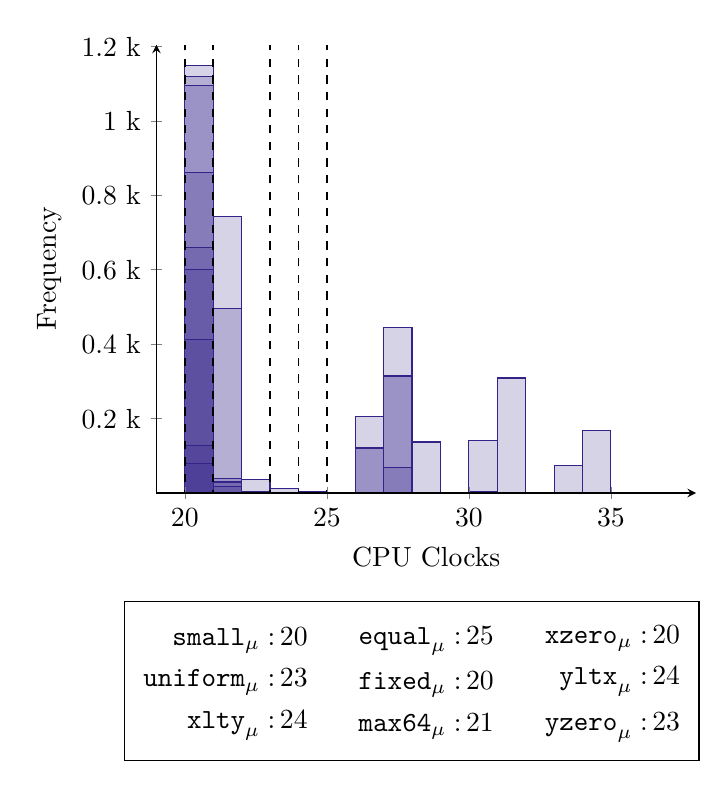
\begin{tikzpicture}[>=latex]
        \begin{axis}[
            axis x line=center,
            axis y line=center,
            name=ax,
            scaled y ticks=base 10:-3,
            ytick scale label code/.code={},
            yticklabel={\pgfmathprintnumber{\tick} k},
            xlabel={CPU Clocks},
            ylabel={Frequency},
            x label style={at={(axis description cs:0.5,-0.1)},anchor=north},
            y label style={at={(axis description cs:-0.1,.5)},rotate=90,anchor=south,yshift=4mm},
            area style,
            ymin=0,
            xmin=19,
            xmax=38,
            ymax=1205
            ]
            \addplot+ [ybar interval,mark=no,color=firstCol,fill=firstCol,fill opacity=0.2] table {
                20 78
21 496
22 35
23 1
24 0
25 0
26 1
27 0
28 0
29 0
30 141
31 309
32 0
33 0
34 1
35 0
36 1
37 1
            };
\addplot+ [ybar interval,mark=no,color=firstCol,fill=firstCol,fill opacity=0.2] table {
                20 1119
21 8
            };
\addplot+ [ybar interval,mark=no,color=firstCol,fill=firstCol,fill opacity=0.2] table {
                20 861
21 17
22 3
23 0
24 0
25 0
26 0
27 69
28 137
29 0
30 1
31 0
32 0
33 0
34 0
35 0
36 0
37 1
            };
\addplot+ [ybar interval,mark=no,color=firstCol,fill=firstCol,fill opacity=0.2] table {
                20 1148
21 10
            };
\addplot+ [ybar interval,mark=no,color=firstCol,fill=firstCol,fill opacity=0.2] table {
                20 659
21 29
22 3
23 0
24 1
25 0
26 122
27 314
28 1
29 1
30 3
31 0
32 0
33 0
34 0
35 0
36 0
37 2
            };
\addplot+ [ybar interval,mark=no,color=firstCol,fill=firstCol,fill opacity=0.2] table {
                20 413
21 39
22 1
23 0
24 3
25 0
26 205
27 445
28 2
29 1
30 0
31 0
32 0
33 0
34 0
35 1
36 0
37 1
            };
\addplot+ [ybar interval,mark=no,color=firstCol,fill=firstCol,fill opacity=0.2] table {
                20 1094
21 11
            };
\addplot+ [ybar interval,mark=no,color=firstCol,fill=firstCol,fill opacity=0.2] table {
                20 128
21 743
22 0
23 13
24 3
25 0
26 0
27 0
28 1
29 2
30 0
31 0
32 0
33 75
34 169
35 0
36 0
37 2
            };
\addplot+ [ybar interval,mark=no,color=firstCol,fill=firstCol,fill opacity=0.2] table {
                20 600
21 32
22 1
23 1
24 1
25 0
26 120
27 315
28 1
29 0
30 1
31 1
32 0
33 0
34 0
35 0
36 0
37 2
            };
                                \draw[color=black, line width=0.2mm, dashed] 
                (axis cs:25, -60.25) -- (axis cs:25, 1205);
                \draw[color=black, line width=0.2mm, dashed] 
                (axis cs:20, -60.25) -- (axis cs:20, 1205);
                \draw[color=black, line width=0.2mm, dashed] 
                (axis cs:21, -60.25) -- (axis cs:21, 1205);
                \draw[color=black, line width=0.2mm, dashed] 
                (axis cs:20, -60.25) -- (axis cs:20, 1205);
                \draw[color=black, line width=0.2mm, dashed] 
                (axis cs:23, -60.25) -- (axis cs:23, 1205);
                \draw[color=black, line width=0.2mm, dashed] 
                (axis cs:24, -60.25) -- (axis cs:24, 1205);
                \draw[color=black, line width=0.2mm, dashed] 
                (axis cs:20, -60.25) -- (axis cs:20, 1205);
                \draw[color=black, line width=0.2mm, dashed] 
                (axis cs:24, -60.25) -- (axis cs:24, 1205);
                \draw[color=black, line width=0.2mm, dashed] 
                (axis cs:23, -60.25) -- (axis cs:23, 1205);
        \end{axis} 
        \node[below=15mm of ax] (1) {
            $\begin{aligned}
                \texttt{equal}_\mu: & \,25\\
                \texttt{fixed}_\mu: & \,20\\
                \texttt{max64}_\mu: & \,21
            \end{aligned}$
        };
        \node[left=4mm of 1] (2) {
            $\begin{aligned}
                \texttt{small}_\mu: & \,20\\
                \texttt{uniform}_\mu: & \,23\\
                \texttt{xlty}_\mu: & \,24
            \end{aligned}$
        };
        \node[right=4mm of 1] (3) {
            $\begin{aligned}
                \texttt{xzero}_\mu: & \,20\\
                \texttt{yltx}_\mu: & \,24\\
                \texttt{yzero}_\mu: & \,23
            \end{aligned}$
        };
        \node[fit=(1)(2)(3),draw]{};
        \end{tikzpicture}%
      \end{lrbox}\resizebox{\textwidth}{!}{\usebox{\mybox}}
      \caption{Fuzzing results visualized. The means of each fuzz class are shown as vertical lines.}
    \end{subfigure}
    \hspace{1cm}
    \begin{subfigure}[b]{0.3\textwidth}
      \begin{lstlisting}[style=defstyle,language={[x86masm]Assembler},basicstyle=\footnotesize\ttfamily,breaklines=true]
...
  pushq	%rbp
  movq	%rsp, %rbp
  movq	%rdi, -8(%rbp)
  movq	%rsi, -16(%rbp)
  cmpq	$0, -8(%rbp)
  js	.L2
  movl	$-29, %eax
  movl	$-37, %edx
  movl	%eax, %ecx
  sarl	%cl, %edx
  movl	%edx, %eax
  cmpl	$1, %eax
  jle	.L3
.L2:
  movl	$1, %eax
  jmp	.L5
.L3:
  movl	$0, %eax
.L5:
  popq	%rbp
  ret
...\end{lstlisting} 
       \caption{Fuzzed assembly code.}
  \end{subfigure}
  \caption{An example of a true positive, i.e. a variable-time program that was rejected by Welch's t-test, from the \texttt{O0} dataset. 
  The source code of the program is shown in Appendix \ref{appendix:general-optimizations-results}. 
  Notice that inputs from the input classes \texttt{small}, \texttt{xzero}, \texttt{fixed} and \texttt{max64} are significantly faster than the rest.
  That is because the program branches on whether $x$ is signed or not (\texttt{js} instruction in line 7), which it never is in these 4 classes.}
  \label{fig:general-optimizations-O0-true-positive}
\end{figure}

Findings from the other datasets also deserve mentioning.
The \texttt{O1}, \texttt{O2}, \texttt{O3} and \texttt{Os} datasets had several false negatives, i.e. programs that were not rejected by Welch's t-test, but were variable-time.
Concretely, we saw examples where the assembled code branched on a \textit{very} specific scenario, e.g. if $x = 8129346172934691$, which is near-impossible to detect by fuzzing since the probability of hitting that specific value is very low.
We did not find any false positives in any other dataset than \texttt{O0}.
This is because the vast majority of programs in the \texttt{O1}, \texttt{O2}, \texttt{O3} and \texttt{Os} datasets were variable-time.
This points to the fact that more aggressive optimizations that introduce conditional branching are more likely to produce actual variable-time machine code.
The reason that Welch's t-test did not detect vulnerabilities in all programs in the datasets is likely due to the above-mentioned false negatives, but also because the t-test has some inherent limitations as mentioned in Section \ref{sec:statistical-analysis}.
Concrete examples of true and false positives and negatives can be found in Appendix \ref{appendix:general-optimizations-results}.

Finally, we want to address the fact that the general optimizations datasets were generated with programs that had ASTs of max depth 5.
This was done to reduce the length of the programs to make them more manageable for analysis.
However, we also generated datasets with ASTs of max depth 12 and found that the results were similar in the \texttt{O0} and \texttt{O1} datasets, while the \texttt{O2}, \texttt{O3} and \texttt{Os} datasets had significantly more programs with conditional branching -- around 5\%, 5\% and 2\% respectively.
We deem the choice of max depth 5 to be a good compromise between the length of the programs and the number of conditional branches since our results underline the problem we are trying to address.

\subsection{Specific Optimizations}
\label{sec:specific-optimizations}
The results in Table \ref{tab:general-optimizations} show that the percentage of vulnerable programs is the highest for the \texttt{O0} dataset, then it decreases significantly for the \texttt{O1} dataset, and then it increases significantly for the \texttt{O2} and \texttt{O3} datasets.
The significant decrease from \texttt{O0} to \texttt{O1} points to the fact that some optimizations in \texttt{gcc} decrease the number of conditional branches. 
Despite running several hundred experiments testing each possible configurable optimization flag \citep{gcc-manual} individually, we were not able to identify which optimizations were responsible for this decrease.
Furthermore, applying all configurable optimizations from \texttt{O1} to \texttt{O0} at once did not result in a decrease in the number of conditional branches.
This points to the fact that the responsible optimizations are non-configurable, i.e. they are always enabled for \texttt{O1}.
This also underlines the fact that all the \texttt{O*} flags enable optimizations that are non-configurable \citep{gcc-manual}, which in turn gives the developer less control over disabling problematic optimizations to increase the security of the code.

The significant increase from \texttt{O1} to \texttt{O2} and \texttt{O3} points to the fact that some optimizations in \texttt{gcc} can introduce conditional branches and therefore timing vulnerabilities. 
We identified a configurable compiler optimization that was responsible for introducing conditional branches in our datasets: \texttt{ftree-pre}.
This optimization performs partial redundancy elimination \citep{gcc-manual}.
\texttt{ftree-pre} is enabled by default for \texttt{O2}, \texttt{O3}, and \texttt{Os}, but not for \texttt{O1}.

Partial redundancy elimination (PRE) is a form of common subexpression elimination (CSE) that tries to eliminate redundant computations. 
We discussed how CSE works and how it can introduce conditional branches in Section \ref{sec:cse}.
Specifically, PRE tries to eliminate computations that are redundant in some, but not all, control flow paths.
This is done by moving the computation to a point in the program where it is guaranteed to be executed only once.
This results in different control flow paths with different amounts of instructions, which in turn result in timing vulnerabilities.

\subsection{Vulnerable Expressions}
\label{sec:vulnerable-expressions}
Finally, we identified various types of expressions that were compiled into conditional branches.
We identified expressions on the form $c$ \texttt{op} $x$ \texttt{comp} $y$, where $c$ is a constant, \texttt{op} is a bitwise operator, \texttt{comp} is a comparison operator, and $x$ and $y$ are variables.
Expressions of this form result in constant-time code containing conditional branches, much like the example in Figure \ref{fig:assembly-inspection-example}.

A more severe type of expression that we identified was expressions on the form $undefined$ \texttt{op} $(x$ \texttt{comp} $y)$, where $undefined$ contains undefined behavior, \texttt{op} is a bitwise operator, \texttt{comp} is a comparison operator, and $x$ and $y$ are variables. 
Expressions of this form sometimes result in variable-time code when compiled with \texttt{O0}.
However, when compiled with \texttt{O1}, \texttt{O2}, \texttt{O3} or \texttt{Os}, the entire program is optimized away and replaced with \texttt{return 0;}.
This is because the compiler can deduce that the expression contains undefined behavior, and, according to the C standard, the compiler is allowed to replace undefined behavior with anything \citep{c-standard}.
An example of this type of expression and its corresponding assembly, when compiled with \texttt{O0}, is shown in Figure \ref{fig:vulnerable-expression}.

\begin{figure}[H]
  \centering
     \begin{subfigure}[b]{0.41\textwidth}
        \begin{lstlisting}[style=defstyle,language={C},basicstyle=\ttfamily,breaklines=true]
int program(long long int x, long long int y) { 
  return (42 >> -1) & (x == y); 
}\end{lstlisting} 
      \vspace{6em}
      \caption{An example of a program containing an expression of the form $undefined$ \texttt{op} $(x$ \texttt{comp} $y)$.
      Specifically, bit-shifting with a negative number is undefined behavior in C \citep{c-standard}.}
    \end{subfigure}
    \hspace{1cm}
    \begin{subfigure}[b]{0.3\textwidth}
      \begin{lstlisting}[style=defstyle,language={[x86masm]Assembler},basicstyle=\footnotesize\ttfamily,breaklines=true]
...
  pushq   %rbp
  movq    %rsp, %rbp
  movq    %rdi, -8(%rbp)
  movq    %rsi, -16(%rbp)
  movq    -8(%rbp), %rax
  cmpq    -16(%rbp), %rax
  jne     .L2
  movl    $-1, %eax
  movl    $42, %edx
  movl    %eax, %ecx
  sarl    %cl, %edx
  movl    %edx, %eax
  andl    $1, %eax
  jmp     .L4
.L2:
  movl    $0, %eax
.L4:
  popq    %rbp
  ret
...\end{lstlisting} 
       \caption{Corresponding assembly code when compiled with \texttt{O0} in \texttt{gcc}.}
  \end{subfigure}
  \caption{An example of a small program that causes \texttt{gcc} to generate variable-time code when compiled with \texttt{O0}. Specifically, one can obtain whether $x$ is equal to $y$ by timing the program.}
  \label{fig:vulnerable-expression}
\end{figure}

Finally, and perhaps most importantly, we identified expressions that will result in variable-time code when compiled with \texttt{O2}, \texttt{O3} and \texttt{Os}.
As mentioned in Section \ref{sec:specific-optimizations}, partial redundancy elimination (PRE) can introduce conditional branches.
PRE is enabled for \texttt{O2}, \texttt{O3} and \texttt{Os} \citep{gcc-manual}.
In some expressions of the form $e$ \texttt{comp} $e'$, where $e$ and $e'$ contain subexpressions that are not common between $e$ and $e'$, PRE will introduce conditional branches. An example of this is shown in Figure \ref{fig:pre-example}.

\begin{figure}[H]
  \centering
  \begin{lstlisting}[style=defstyle,language={C},basicstyle=\ttfamily,breaklines=true, xleftmargin=3cm, xrightmargin=3cm]
int program(long long int x, long long int y) { 
  return 42 * (x == 42) == (y == 42); 
}\end{lstlisting} 
    \caption{An example of a program that will be variable-time when compiled with \texttt{O2}, \texttt{O3} or \texttt{Os}, specifically because of PRE.
    PRE will identify two control flow paths in this expression: 
    One where $x=42$ and one where $x \neq 42$.
    If $x=42$, the expression will always evaluate to $0$ since \texttt{42 * (42 == 42) == (y == 42)} will evaluate to $42 \stackrel{?}{=} 0$ or $42 \stackrel{?}{=} 1$ which is false in both cases.
    If $x \neq 42$, the expression depends on whether $y=42$.
    Hence \texttt{(y == 42)} is redundant in the first control flow path, but not in the second.
    As a result, PRE will insert a conditional branch that branches on $x = 42$ and only considers $y$ if that is \textit{not} the case.}
    \label{fig:pre-example}
\end{figure}


\section{Evaluation}
\todo{Evaluation of OptiFuzz and analysis. Is it accurate?}

\todo{From results, we can see that most programs with conditional branches are rejected by the t-test.
This means that our underapproximation by the inspection is okay.}

\section{Discussion}
From the previous sections, it is clear that modern compilers introduce timing vulnerabilities in constant-time programs.
This is devastating for security since it means that developers cannot reliably write constant-time code.
A solution is required.
In this section, we discuss how the problem can be solved and what the implications different solutions have on security and efficiency.

As shown in Section \ref{sec:gcc-vs-clang}, \texttt{clang} is much more conservative when it comes to inserting conditional branches in constant-time programs.
Instead of inserting variable-time conditional branches, \texttt{clang} uses constant-time conditional moves to implement branching control flow.
From this observation, it might be tempting to conclude that always substituting conditional branches with conditional moves is the solution to the problem.
However, there is more to the story.

\texttt{cmov} instructions severely restrict the out-of-order engine on modern CPUs since \texttt{cmov} instructions increase the data dependency between instructions significantly \citep{intel-optimization-reference}. 
Furthermore, branch predictions are not used for \texttt{cmov} instructions, which can lead to significant performance degradation.
Hence, we have to address this trade-off between security and efficiency.

\subsection{Forcing \texttt{cmov} Instructions When Necessary}
This trade-off between security and efficiency has led multiple researchers to propose solutions that only force \texttt{cmov} instructions to be used on critical data \citep{what-you-c,llvm-issues-blog-post}.
In both studies, the authors propose to add the possibility to specify forced \texttt{cmov} instructions in the source code and restrict the backend of the compiler to not being able to optimize the \texttt{cmov} away for those specific instructions.
This solution has the advantage that it does not affect the performance of non-critical parts of the program.
In fact, \citeauthor{what-you-c} show that their solution only introduces a performance penalty of 1\% and sometimes even increases performance.

However, this solution also has its disadvantages.
First, the solution relies heavily on the developer.
The developer has to know which parts of the program are critical, and also be able to use the language extension correctly.
In turn, it means that security relies on human factors, which are error-prone.
Second, the solution relies on the compiler being configurable to avoid forced \texttt{cmov} instructions being optimized away.
As we discussed in Section \ref{sec:gcc-vs-clang} and \ref{sec:general-optimizations}, \texttt{clang} seems to be quite configurable while \texttt{gcc} does not.
Hence, the solution might not be easily applicable to all compilers.

Another solution is to implement vulnerable parts of the program using a domain-specific language that is designed to be constant-time.
\citeauthor{fact} proposed a domain-specific language, called FaCT, for implementing constant-time cryptographic algorithms \citep{fact}.
FaCT is designed to be interoperable with C, and the compiler ensures constant-time code by leveraging the \texttt{ct-verif} tool that is based on verification of the LLVM IR \cite{verifying-constant-time-llvm}.
\texttt{ct-verif} operates on a formalization of constant-time code and verifies based on a theoretically sound and complete methodology.
However, \citeauthor{verifying-constant-time-llvm} note that the verification process of \texttt{ct-verif} is not guaranteed to identify all timing vulnerabilities due to translation between the LLVM IR and machine code, and due to possible incompleteness of their formalization of constant-time code. 
Some of these issues were experimentally verified.
However, generally \texttt{ct-verif} captures significantly more timing vulnerabilities than other verification alternatives \citep{verifying-constant-time-llvm}.
Additionally, \texttt{ct-verif} is efficient at verifying constant-time code, often being much faster than the compilation step, but occasionally being a few times slower.

\subsection{Bullet-proofing the Compiler}
A more radical approach is to force the compiler to always produce constant-time code.
\citeauthor{verified-constant-time-c-comiler} provides a formally verified constant-time C compiler, built on top of the CompCert verified C compiler \citep{verified-constant-time-c-comiler}. 
The constant-time CompCert compiler guarantees that constant-time source code is compiled into constant-time machine code.
This is achieved by instrumenting the operational semantics of CompCert's IR to be able to capture cryptographic constant-time and proving that cryptographic constant-time is preserved during compilation. 
This has immense advantages for security.

However, the security advantages come at the cost of efficiency. 
The constant-time CompCert compiler is significantly slower than \texttt{gcc}.
Experimental results show an efficiency penalty of well over 100\% in some cases \citep{verified-constant-time-c-comiler}.

\subsection{Testing Solutions}
The final category of solutions we identified is black-box testing solutions like DudeCT \citep{dudect} and our tool OptiFuzz.
Concretely, one can test specific implementations for timing vulnerabilities using these tools.
These tests can even be automated to run as part of a continuous integration pipeline.
Solutions in this category have the obvious advantage that they are simple and require no modeling of hardware behavior or language semantics.
It is arguably the most practical solution since it does not require any changes to the compiler or the language.
It also does not induce any performance penalty.

The testing solutions, however, come with a significant security disadvantage in that they are noisy and not exact.
As we showed in Section \ref{sec:general-optimizations}, OptiFuzz will produce false positives and false negatives.
\citeauthor{dudect} raised similar concerns for DudeCT.
Fuzzing tools provide more of an indication of the presence of timing vulnerabilities than a guarantee.

\todo{Argue that many solutions exist with a mixture of security and efficiency.
We argue that people should start using them.
Perhaps OptiFuzz + compromise solutions}

\section{Conclusion and Future Work}
We have a lot of ideas for future work that we did not get around to. These include:
\begin{itemize}
    \setlength\itemsep{-0.6em}
    \item Extend OptiFuzz to generate more complicated programs, eg. by reintroducing the division and modulus operators while dealing with division by zero in a meaningful way.
    \item Increasing the precision of the assembly inspection. One way could be to detect if branches contain the same amount of work and identify them as constant time.
    \item Implement other relevant input classes. A dynamic class containing the hardcoded values from a program. This might be able to catch the very specific but unpredictable values that courses branching.
    \item Extending the usage of Welsh's t-test to all classes, and not just between \texttt{uniform} and \texttt{fixed}.
    \item Create a tool that warns developers in real-time about constant C expressions that might be compiled to variable time by comparing it to a database precomputed using OptiFuzz. This tool could furthermore be implemented in a CI/CD environment.
    \item Extend OptiFuzz to support other processor architecture, especially including ones used by embedded systems.
\end{itemize}


\pagebreak

\bibliographystyle{abbrvnat}
\bibliography{litterature}

\pagebreak
\begin{appendices}

\section{Select General Optimizations Results}
\label{appendix:general-optimizations-results}
%\documentclass[10pt]{article}
\usepackage[left=0.8in,right=0.8in,bottom=0.5in,top=0.5in]{geometry}
\geometry{a4paper}
\usepackage[parfill]{parskip}    % Activate to begin paragraphs with an empty line rather than an indent
\usepackage{graphicx}
\usepackage{xcolor}
\usepackage{hyperref}
\usepackage{titling}
\usepackage[small,compact]{titlesec}
\usepackage[toc,page]{appendix}

\usepackage{listings}
\usepackage{pgfplots}
\usepackage{adjustbox}
\usepackage{float}
\usepackage{subcaption}
\usepackage{pgffor}
\usepackage{expl3}
\usepackage{xparse}
\usepackage{xfp}
\usetikzlibrary{fit}
\usetikzlibrary{positioning}


\usepackage{amsmath,amssymb}
\DeclareGraphicsRule{.tif}{png}{.png}{`convert #1 `dirname #1`/`basename #1 .tif`.png}



\newcommand\courseName{Language-Based Security}
\newcommand\courseNameAbbrv{LBS}
\newcommand\courseYear{2023}
\newcommand\courseAndYear{\courseNameAbbrv-\courseYear}
\newcommand\reportKind{Exam Report}

\newcommand\groupNumber[1]{
  \makeatletter
  \def\@courseGroupNumber{#1}
  \makeatother
}

\pretitle{\begin{flushright} \bfseries  \large \courseAndYear: \reportKind \end{flushright}   \begin{flushleft}
\bfseries \LARGE}
\posttitle{\par\end{flushleft}\vskip 0.5em}

\preauthor{
\begin{flushleft}
\large \lineskip 0.5em%
\bfseries
\makeatletter Group \@courseGroupNumber \\ \makeatother
\begin{tabular}[t]{@{}l}}
\postauthor{\end{tabular}\par\end{flushleft}}

\predate{\begin{flushleft}\bfseries \large}
\postdate{\par\end{flushleft}}

\usepackage{listings}
\usepackage{pgfplots}
\usepackage{adjustbox}
\usepackage{float}
\usepackage{subcaption}
\usepackage{pgffor}
\usepackage{expl3}
\usepackage{xparse}
\usepackage{xfp}

\newcommand\todo[1]{\textcolor{red}{TODO: #1}}

\pgfplotsset{compat=1.12}

\definecolor{mGreen}{rgb}{0,0.6,0}
\definecolor{mGray}{rgb}{0.5,0.5,0.5}
\definecolor{mPurple}{rgb}{0.58,0,0.82}
\definecolor{backgroundColour}{rgb}{0.95,0.95,0.92}

\definecolor{firstCol}{HTML}{332288}
\definecolor{secondCol}{HTML}{117733}
\definecolor{thirdCol}{HTML}{44AA99}
\definecolor{fourthCol}{HTML}{88CCEE}
\definecolor{fifthCol}{HTML}{DDCC77}
\definecolor{sixthCol}{HTML}{DD2255}

\lstdefinestyle{defstyle}{
    backgroundcolor=\color{backgroundColour},   
    commentstyle=\color{mGreen},
    keywordstyle=\color{magenta},
    numberstyle=\tiny\color{mGray},
    stringstyle=\color{mPurple},
    basicstyle=\footnotesize,
    breakatwhitespace=false,         
    breaklines=true,                 
    captionpos=b,                    
    keepspaces=true,                 
    numbers=left,                    
    numbersep=5pt,                  
    showspaces=false,                
    showstringspaces=false,
    showtabs=false,                  
    tabsize=2
}

\newsavebox{\mybox}

\ExplSyntaxOn
\cs_new:Npn \__afp_ismember_loop:Nnw #1#2#3,
  {
    \quark_if_recursion_tail_stop_do:nn {#3}
      { \prg_return_false: }
    #1 {#2} {#3}
      { \use_i_delimit_by_q_recursion_stop:nw { \prg_return_true: } }
      { \__afp_ismember_loop:Nnw #1 {#2} }
  }
\prg_new_conditional:Npnn \afp_int_ismember:nn #1#2 { p, T, F, TF }
  {
    \__afp_ismember_loop:Nnw \__afp_int_isequal:nnTF {#1} #2 ,
    \q_recursion_tail , \q_recursion_stop
  }
\prg_new_conditional:Npnn \__afp_int_isequal:nn #1#2 { p, T, F, TF }
  {
    \int_compare:nNnTF {#1} = {#2}
      { \prg_return_true: }
      { \prg_return_false: }
  }
\NewExpandableDocumentCommand { \IncludeExperimentResults } { m m }
  {
    \foreach \x in {1,...,#1} {
        \noindent\bool_if:NF { \afp_int_ismember_p:nn {\x} {#2} } {\input{generated_latex/prog\x.tex}}
    }
  }
\ExplSyntaxOff
\usepackage[authoryear]{natbib}

\title{
  Optimizing Away Security in C
}

\groupNumber{10}
\author{Anders B. Clausen \and Johan T. Degn \and Jonathan Eilath}

\begin{document}
\maketitle
\thispagestyle{empty}

\section*{Abstract}
\todo{After the paper is done}

\section{Introduction}
The C programming language is one of the most widely used programming languages in the world. 
It is used in a wide variety of applications, ranging from embedded systems to cryptographic libraries. 
However, C is also notorious for lacking security guarantees.
Security-related issues in programs written in C stem from both the programmer, but also from the compiler.

The problem with security issues introduced by the compiler is especially prevalent in the context of timing attacks on cryptographic algorithms. 
Developers try to mitigate timing attacks by writing constant-time code -- code where the execution time is independent of the input.
However, the compiler may introduce timing leaks by optimizing away the constant-time code.
In a recent study \citep{developer-survey-timing-attacks}, it was shown that the vast majority of developers of cryptographic libraries rely on constant-time code practices that in theory result in constant-time code, but may be vulnerable after compilation.

The issue of timing vulnerabilities introduced by compilers is well-known in the community.
Several proposals have been made to mitigate the issue \citep{what-you-c, dudect, fact, verified-constant-time-c-comiler}.
However, the problem persists and to the best of our knowledge, no study has quantified the issue of timing vulnerabilities introduced by compilers.

In this paper, we try to quantify the issue of timing vulnerabilities introduced by the two most popular C compilers, gcc\footnote{\url{https://gcc.gnu.org/}.} and clang\footnote{\url{https://clang.llvm.org/}.}.
We do this by implementing a tool, OptiFuzz, that generates, analyzes and fuzzes random C programs.
For simplicity, the generated programs are limited to only containing non-branching arithmetic, logical and comparison operations.
Also \texttt{/} and \texttt{\%} are avoided, to mitigate division-by-zero errors.
We investigate what optimization flags are responsible for introducing timing leaks and compare them.
Finally, we discuss how the issue of timing vulnerabilities introduced by the compiler can be mitigated by using language-based security techniques.

\subsection{Related Work}
The issue of timing vulnerabilities introduced by the clang C compiler across different versions has been researched by Simon et. al. \citep{what-you-c}. 
Several studies have investigated potential solutions to the issue, including using constant-time branching instructions \citep{what-you-c}, using black-box testing software \citep{dudect}, domain-specific languages \citep{fact}, and notably a verified constant-time C compiler has been developed \citep{verified-constant-time-c-comiler}.

\subsection{Contributions}
We provide a quantitative analysis of timing vulnerabilities introduced by gcc and clang, focusing on specific troublesome optimization flags.
Additionally, we provide a tool, OptiFuzz, that can be used to generate, analyze and fuzz random C programs for further investigation of the issue.
\todo{Might be more when we finish the paper}
\subsection{Overview}
This paper is organized as follows: $\ldots$ 
\todo{After we have finished the rest of the paper}
\todo{Insert guide on how to read appendix here??}

\section{Preliminaries}
\subsection{Timing Attacks}
Timing attacks are a class of side-channel attacks that exploit the fact that the execution time of a program can depend on the input.
The history of timing attacks goes back several decades where Kocher showed multiple successful timing attacks on well-known cryptographic algorithms such as Diffie-Hellman and RSA \citep{1996-timing-attacks}.
An example of vulnerable code is shown in Figure \ref{fig:timing-attack-example}.
\begin{figure}[H]
  \begin{lstlisting}[style=defstyle,language=C, xleftmargin=6.8cm, xrightmargin=6.8cm]
int foo(int x) {
  if (x < 100) {
    x *= 2;
    x += 7;
  }
  return x;
} \end{lstlisting} 
  \caption{Example of a program vulnerable to a timing attack. 
  Only by analyzing the execution time of the machine code, an attacker can infer whether the input is less than 100 or not.}
  \label{fig:timing-attack-example}
\end{figure}

\subsection{Optimizing Compilers}
Cryptographers will avoid code like the example in Figure \ref{fig:timing-attack-example} and write constant-time code instead.
Constant-time code is code where the execution time is independent of the input.
However, the compiler may introduce timing vulnerabilities through optimizations by adding variable-time branches to the machine code.
The issue arises in the analysis and transformation phases of the compiler as illustrated in Figure \ref{fig:optimizing-compiler-pipeline}.

\begin{figure}[H]
  \centering
  \input{tikz/optimizing-compiler-pipeline.tex}
  \caption{The pipeline of an optimizing compiler. After the transformation phase, the IR is optimized and the compiler may have introduced timing vulnerabilities.}
  \label{fig:optimizing-compiler-pipeline}
\end{figure}

Many different kinds of optimization techniques are carried out by optimizing compilers, some of which can introduce timing vulnerabilities.
Some common optimization techniques like common subexpression elimination and strength reduction have been shown to introduce timing vulnerabilities \citep{optimizations-linked-to-timing-attacks}.
To illustrate this point, we look at how common subexpression elimination can introduce timing vulnerabilities.

\subsubsection{Timing Vulnerabilities Through Common Subexpression Elimination}
Common Subexpression Elimination is an optimization technique that extracts subexpressions that are common across multiple expressions and replaces them with a single variable.
This optimization technique can introduce timing vulnerabilities since it can decrease the number of instructions executed for a specific branch of the code as illustrated in Figure \ref{fig:common-subexpression-elimination}.
Here the common subexpression \texttt{2 * 3 + 5} is extracted and assigned to the variable \texttt{common}, making the \texttt{else} branch execute faster than the \texttt{if} branch.

\begin{figure}[H]
  \centering
     \begin{subfigure}[b]{0.3\textwidth}
        \begin{lstlisting}[style=defstyle, language=C]
int foo(int x, int *arr) {
  if (x == SECRET) {
    x = arr[0] * 3 + 5;
    x += arr[1] * 3 + 5;
    x += arr[2] * 3 + 5;
  } else {
    x = 2 * 3 + 5;
    x += 2 * 3 + 5;
    x += 2 * 3 + 5;
  }
  return x;
} \end{lstlisting} 
         \caption{Original code.}
    \end{subfigure}
    \hspace{1cm}
    \begin{subfigure}[b]{0.3\textwidth}
      \begin{lstlisting}[style=defstyle, language=C]
int foo(int x, int *arr) {
  if (x == SECRET) {
    x = arr[0] * 3 + 5;
    x += arr[1] * 3 + 5;
    x += arr[2] * 3 + 5;
  } else {
    // optimized
    int common = 2 * 3 + 5;
    x = 3 * common;
  }
  return x;
} \end{lstlisting} 
       \caption{Optimized code.}
  \end{subfigure}
  \caption{An example of how the common subexpression elimination can introduce timing vulnerabilities in code. (a) shows the original code and (b) shows the optimized code.}
  \label{fig:common-subexpression-elimination}
\end{figure}

\section{OptiFuzz}
We created a tool, OptiFuzz, that can be used to generate, analyze and fuzz random C programs.
The source code for OptiFuzz is available on GitHub\footnote{\url{https://github.com/anbclausen/optifuzz}.}.
The goal of OptiFuzz is to quantify the issue of timing attacks introduced by C compilers with different optimization flags enabled.
The tool works as follows:
\begin{itemize}
  \item OptiFuzz generates random C programs consisting of non-branching arithmetic, logical and comparison operations.
  \item OptiFuzz then compiles the generated C programs with different specified optimization flags enabled and inspects the generated assembly for branching instructions introduced by the compiler.
        If branching is found, the program is flagged.
  \item OptiFuzz then fuzzes the flagged programs with various random inputs to test whether the branching instructions can be exploited to leak information about the input.
  \item At last, OptiFuzz reports the results of the fuzzing in the form of a PDF report.
\end{itemize}
The OptiFuzz pipeline is illustrated in Figure \ref{fig:optifuzz-pipeline}. 
Each of the steps in the pipeline is described in detail in the following sections.
\begin{figure}[H]
  \centering
  \input{tikz/optifuzz-pipeline.tex}
  \caption{The OptiFuzz pipeline.}
  \label{fig:optifuzz-pipeline}
\end{figure}




\subsection{Code Generation}
The first step in the OptiFuzz pipeline is code generation. 
The code generation module is written in OCaml and works by generating abstract syntax trees according to the grammar in Figure \ref{fig:grammar}.

\begin{figure}[H]
  \centering
  \begin{align*}
    e \in Expr ::= & x \mid y &\text{(input variables)}\\
    & n \in \{0, 1\}^{64} &\text{(64-bit integer literals)}\\
    & -e \mid e + e \mid e - e \mid e \times e &\text{(arithmetic operators)}\\
    & \texttt{true} \mid \texttt{false} &\text{(boolean literals)}\\
    & !e &\text{(logical operators)}\\
    & e < e \mid e \leq e \mid e > e \mid e \geq e \mid e = e \mid e \neq e &\text{(comparison operators)}\\
    & e \texttt{\&} e \mid e \texttt{|} e \mid \text{\~{}} e \mid e \text{\^{}} e \mid e \ll e \mid e \gg e &\text{(bitwise operators)}
  \end{align*}
  \caption{The grammar that defines the ASTs generated by the code generation module in the OptiFuzz pipeline.}
  \label{fig:grammar}
\end{figure}

The grammar defines all programs with 2 variables and non-branching arithmetic, logical and comparison operations in C \citep{c-standard}, excluding division (\texttt{/}) and modulus (\texttt{\%}).
The reason for excluding division and modulus is that they may cause division-by-zero errors.
Generated programs are forced to include both input variables, $x$ and $y$.
$x$ and $y$ are the inputs to the program, and we require both to be present since programs with 0 or 1 input variables are trivially constant-time.
An example of a program generated by the code generation module is shown in Figure \ref{fig:code-gen-example}.

\begin{figure}[H]
  \begin{lstlisting}[style=defstyle,language=C, xleftmargin=2.7cm, xrightmargin=2.7cm]
#define false 0
#define true 1
int program(int x, int y) { return !(y * (43 * (x != true))); } \end{lstlisting}
  \caption{Example of a program generated by the code generation module.}
  \label{fig:code-gen-example}
\end{figure}

The code generation module works by generating a random distribution that selects different symbols in the grammar with a certain probability.
This ensures that not all generated programs will be uniformly random.
For example, if a generated distribution heavily favors the left-shift operator, then the generated programs will contain a lot of left-shift operations.
This is useful for detecting whether certain types of programs are more likely to be constant-time than others.

The code generation module generates programs with integer literals in different ranges. 
Booleans represent the first range.
Defining Booleans as integers is a common practice in C \citep{c-standard}.
Integers from this range are included since the constants 0 and 1 are interesting in many operations.
The second range we consider is $[0, 64]$ as numbers in this range are lower than the size of 64-bit integers.
Hence numbers in this range are interesting in bit-shifting operations.
The third range is the range of signed 64-bit integers.
Generally, we have included these smaller ranges of integers since they are interesting and it is very unlikely that a uniformly random 64-bit integer would be in these ranges.

The grammar in Figure \ref{fig:grammar} generates programs with undefined behavior.
For example, bit-shifting with a negative number, or a number larger than the size of the type, is undefined behavior in C \citep{c-standard}.
We chose to include undefined behavior in the grammar since it is a source of timing vulnerabilities \citep{what-you-c}, and it is common in real-life code \citep{undefined-behavior-c}.
The grammar also does not distinguish operations on Booleans and integers and hence generates untypical C programs.
For example, the program in Figure \ref{fig:code-gen-example} features multiplication between a Boolean and an integer.
We chose to include this in the grammar since it is a used trick to avoid branching in constant-time code \citep{what-you-c}.

\subsubsection{Limitations}
The biggest limitation of this approach is that the generated programs are not representative of real-life code since they use such a limited subset of the C language.
However, as argued above the simple constant-time programs are representative of how real code might look, and thus gives a useful insight into the issue of timing vulnerabilities introduced by the compiler.
\subsection{Assembly Inspection}
\label{sec:inspection}

The next step in the OptiFuzz pipeline is assembly inspection.
The assembly inspection module is written in Python and works by inspecting the assembly generated by the compiler across different optimization flags.
The compiled assembly is inspected for conditional branching instructions and flagged if that is the case.
The assembly inspection module is only able to analyze x86-64 assembly.

In x86-64 assembly, \texttt{Jcc} (note, this does not include \texttt{JMP}), \texttt{LOOP} and \texttt{LOOPcc} are the only conditional branching instructions \citep{intel-reference}.
This means that the assembly inspection module only needs to look for these instructions.
Both \texttt{Jcc} and \texttt{LOOPcc} refer to a family of instructions where \texttt{cc} is a condition code.
For example, \texttt{JE} (jump if equal) is in the \texttt{Jcc} instruction family. 
We did not include conditional move instructions in the analysis since they are constant-time \citep{cmov-is-constant-time}.

\subsubsection{Limitations}
An obvious limitation of this approach is that it is tailored for x86-64 assembly.
Hence our analysis will not work for other architectures.
Furthermore, the programs that are flagged by the assembly inspection module are not necessarily vulnerable to timing attacks.
Hence, the assembly inspection module overapproximates the set of programs that are vulnerable to timing attacks.
For example, the program in Figure \ref{fig:assembly-inspection-example} is flagged by the assembly inspection module, but it is constant-time since both branches take the same amount of time to execute.

\begin{figure}[H]
  \centering
  \begin{lstlisting}[style=defstyle, language={[x86masm]Assembler}, basicstyle=\footnotesize\ttfamily,breaklines=true, xleftmargin=4cm, xrightmargin=4cm]
...
  cmpl    $1, -4(%rbp) ; compare TOS to 1
  je      .L2          ; jump to .L2 if equal
  movl    $43, %eax    ; move 43 into %eax
  jmp     .L3
.L2:
  movl    $0, %eax     ; move 0 into %eax
.L3:
  ret\end{lstlisting}
  \caption{Example of a program that is flagged by the assembly inspection module, but is constant-time.}
  \label{fig:assembly-inspection-example}
\end{figure}
\subsection{Fuzzing}
After the assembly inspection has performed the static analysis and flagged programs with potential timing vulnerabilities, the next step is to run a dynamic analysis on them to try and confirm their presence. For this, we have created a fuzzer that runs the programs compiled with the specified compiler and optimization levels fuzzing the arguments the program takes as inputs and measuring its execution time. 

The process goes as follows. First, the fuzzer itself is compiled into object files which are not yet linked. This compilation only needs to happen once. Each of the programs flagged by the static assembly analysis is then compiled one at a time with the specified compiler for each of the supplied optimization flags and linked with the pre-compiled fuzzer. This includes the flags for which the assembly inspector did not detect any branches. This creates a complete fuzzer including the program to fuzz.

The fuzzer generates inputs according to fuzzing classes. For each input it chooses a uniformly random class among the supplied ones. This way there is no biased order in which the inputs from different classes are used, and thus potential noise is likely to effect all classes equally. This is important when comparing timing distributions in the following analysis. After generating the inputs it runs through them and calls the internally linked program with each of them. The programs' execution time is measured every time it is run. The fuzzer repeats the run-through multiple times (50) to allow for detection of outliers and get as precise results as possible. Note that an input is only repeated after each of the others and not multiple times in a row. In addition to having a random class input order, this ensures that any noise that results in longer execution times are not concentrated on a few inputs but distributed over all (or many) of them. This way we minimize the chance of falsely identifying an input or class of inputs as the course of a longer execution time.

As mentioned we use different classes for the inputs to the fuzzer, instead of always generating completely random numbers. This is done to try and capture variable execution time that only takes place a small sample of the values. This could as an example be if there is a check for if one of the inputs are zero. If we only used uniformly random 64-bit numbers it would be unlikely to observe it happen. Even if it did, it would probably just be filtered out as an outlier. Hence, the need for fuzzing classes. For each input there are an $x$ and a $y$ value. The classes the following generates inputs with respect to $x$ and $y$ as seen in the following list.
\begin{itemize}
    \item UNIFORM: They are uniformly random 64-bit numbers.
    \item EQUAL:   They have the same uniformly random 64-bit number.
    \item MAX64:   A random one is a random 64-bit number, the other is uniformly random.
    \item XZERO:   $x$ is 0, $y$ is a uniformly random number.
    \item YZERO:   $y$ is 0, $x$ is a uniformly random number.
    \item XLTY:    Two uniformly random numbers are generated, $x$ is set to the smaller, $y$ to the larger.
    \item YLTX:    Two uniformly random numbers are generated, $y$ is set to the smaller, $x$ to the larger.
    \item SMALL:   They are uniformly random 8-bit numbers (the upper 56 bits are set to 0).
    \item FIXED:   They have the same fixed number $0x12345678$ (used for the T-test).
\end{itemize}
These classes have been made based on observations of values commonly used in comparison in the assembly.

Precise measurements of a program's execution time is not trivial. It can be influenced by a number of things including context switches, interrupts, out-of-order execution, varying CPU clock speed and congestion. Furthermore, since we are dealing with quite small programs that are quick to run, our options for timing them are reduced. The most obvious way to time a program is using the system clock. But when testing it, it became clear that its resolution was too low. We ended up using the Time Stamp Counter (TSC) which is a high resolution counter that (on newer machines) increase at a fixed rate independent of processor frequency. This method is heavily inspired by the suggestions and results from an Intel white paper \citep{intel-benchmark-code-execution}.
Using the TSC as a reference for time is the best we can do on our x86-64 architecture machine.
This approach also allowed us to avoid the timings being skewed by the CPU performing out-of-order execution. Out-of-order could lead to the instructions being reordered resulting in not reading the TSC (with the RDTSC(P) instruction) at the exact time we want to. This is done by utilizing the non-privileged CPUID instructions serializing capabilities that ensure that memory transactions for previous instructions are completed before the next instruction is executed \citep[a]{intel-reference}.

When later using these results in the analysis, we use the minimum time for all executions with the same input. Using the minimum time as the true execution time instead of the mean filters out the noise from outliers that are the results of i.e. context-switches or congestion, as argued in \citep{robust-benchmarking}. In comparison to the DudeCT black-box testing program from \citep{dudect}, which just removes top 5\% of the longest measured execution times to reduce such noise, our approach is not prone to accidentally removing measurements of large execution times that are correct and not the result of noise.

\subsubsection{Limitations}
As mentioned in the assembly inspection section, the inspector over approximates and might flag programs which are in fact constant time. Furthermore, we run the fuzzer for all flags if just one of them was flagged by the inspector.
Considering this, we consider the fuzzer successful when it is able to consistently measure clear differences in execution time of a program with respect to its inputs. Such time difference makes it possible to make an educated guess on what the given inputs look like, and hence opens up for a potential timing based side channel attack. This does indeed indicate that the program is vulnerable.

If, on the other hand, the results of this analysis fails to indicate obvious timing differences, then it is not safe to assume that it is then constant time. This of course could be the case since the assembly inspection over approximates. Since fuzzer is conservative and under approximates, it could be that the input classes used in fuzzing where not able to capture the event coursing the variable time. Considering it could also be constant time, we have to settle with not knowing for sure.

Even with the actions taken to get as precise timings as possible the analysis is still prone to some noise. Specifically, it is worth noting that when running this in userland the fuzzer could be influenzed by interupts and preemtion. Both of these requires the code to run in kernel space to disable, which is a possible future extension of the fuzzer. As a compromise making it this less of a source of noise the fuzzer can be run with higher priority, as is the case for our results. 

\subsection{Statistical Analysis}
\label{sec:statistical-analysis}
At the end of the pipeline, we have at our disposal flagged C programs, which have been fuzzed and timed. Now we have to conclude whether or not these programs are variable-time or not. This is a very complex task, as a lot of factors can affect this. Notably, the research conducted by \citeauthor{Abel19a} demonstrates the difficulty of this, as determining the performance of instructions is very microarchitecture dependant. Additionally, \cite{verifying-constant-time-llvm}'s work suggests that static analysis on LLVM can be done, but again suffers from architecture-specific modeling. Thus, we determined that our method should not consider all the intricate details of architecture-specific implementations. Instead, a statistical approach was deemed more suitable.

One statistical approach is to apply significance tests between classes of fuzzing inputs. If we can detect a difference in time between different kinds of inputs, then we can conclude with good probability, that the program is not constant-time. Ideally, for constant-time programs, we would expect a univariate Gaussian with low variation when we measure the running time of the program for all kinds of inputs. Likewise, ideally, for variable-time programs, we hope to see a mixture distribution composed of two (or more) Gaussians with different means. For instance, if we observe two means: $\mu_1 \neq \mu_2$, then we can conclude with good probability, that most likely a branching instruction on the input dictates whether or not the program will have a running time close to $\mu_1$ or $\mu_2$.

\pgfmathdeclarefunction{gauss}{2}{%
  \pgfmathparse{1/(#2*sqrt(2*pi))*exp(-((x-#1)^2)/(2*#2^2))}%
}

% Solution to when the first gaussian is eq to second gaussian plotted in subfigure b)
\def\gausssolution{5.170045172}
\begin{figure}[H]
\captionsetup[subfigure]{justification=centering}
\begin{subfigure}[t]{0.50\textwidth}
\resizebox{\linewidth}{!}{
    \input{tikz/gauss-constant.tex}
}%
\caption{A constant-time program yielding\\a univariate Gaussian with $\mu = 4$.}
\label{fig:univargauss}
\end{subfigure}
\begin{subfigure}[t]{0.50\textwidth}
\resizebox{\linewidth}{!}{
    \input{tikz/gauss-variable.tex}
}%
\caption{A variable-time program, yielding a mixture\\distribution composed of two Gaussian distributions\\having means: $\mu_1 = 4, \mu_2 = 6$ with different variances.}
\label{fig:mixdisgauss}
\end{subfigure}
\caption{An example of what we would expect in theory, when we fuzz constant-time and variable-time programs.}
\label{fig:fuzzclass-statistics-example}
\end{figure}
As seen above in Figure \ref{fig:univargauss}, we have an example of what we, in theory, would think the clock-cycles distribution for a constant-time program would look like. Likewise, Figure \ref{fig:mixdisgauss} shows what the distribution could look like for a variable-time program.

Wishing our measurements will yield such distributions, and then detecting timing leakage is, however, not as simple as described above. \citeauthor{Coron_2004} introduced significance test techniques in general leakage detection; including both timing and power consumption leakage attacks. In the paper, they argue that there is a correlation between measured time and external parameters \citep{Coron_2004}. As an illustrative example, we could use input class A for 10 minutes followed by 10 minutes of fuzzing with input class B while recording the corresponding timing outcomes. It is important to consider that the 10-minute duration of fuzzing with class A might have triggered certain system mechanisms such as a built-in thermal throttle for the CPU, resulting in a reduction of processing speed. Consequently, when evaluating the second input class B it may exhibit a distinct mean value due to the altered conditions induced by the previous measurements. There are a lot of external events to consider that might introduce noise to our data -- so the authors' suggested guideline is to alternate between classes when we measure. This essentially makes sure that the external noise is equally applied to both classes.

The previously mentioned tool in \ref{sec:fuzzing}, DudeCT, by \citeauthor{dudect} works in the above fashion. They, however, extended \citeauthor{Coron_2004}'s approach, by not only interleaving the input classes but by randomly choosing one. According to the authors, this should further reduce noise.

%%%%%%%%%%%%
% PR TODO:
% I believe, even though this is something in the fuzzer,
% that it makes sense to have it in this section, as it fits 
% beautifully with the theory presented, which finally leads to our methodology
%%%%%%%%%%%%
Our methodology extends the above, where we further try to reduce noise, by fuzzing multiple times and picking the minimum measured time. This is visualized in Figure \ref{fig:noisered} below. 
\begin{figure}[H]
    \centering
    \input{tikz/stat-fuzzing_method.tex}
    \caption{Noise reduction by picking the minimum measurement of multiple runs.}
    \label{fig:noisered}
\end{figure}
For example, if we in our random class sequence \{A, B, B, C\} do two iterations:
\begin{center}
    \{A: 2, B: 3, B: 5, C: 2\} \\
    \{A: 4, B: 3, B: 4, C: 3\}
\end{center}
where A: 2 corresponds to the program given input from input class A took 2 clock cycles to run, then the final saved measurements would be: \{A: 2, B: 3, B: 4, C: 2\}. Note that the random class sequence samples once and fixes the input for all iterations.

Using the minimum time as the true execution time instead of the mean filters out the noise from outliers  \citep{robust-benchmarking}.
In comparison to DudeCT by \citeauthor{dudect}, which just removes the top 5\% of the longest measured execution times to reduce such noise, our approach is not prone to accidentally removing measurements of large execution times that are correct and not the result of noise.

Now we apply a significance test to our measurements. There is a great consensus that Welch's t-test \citep{WELCH1947} works great for the task of leakage detection \citep{cryptoeprint:2015/536}.
The test tests the null hypothesis that two populations have equal means, which aligns exactly with our described objectives. The strengths of utilizing Welch's t-test are that it is robust to different variances as seen in figure \ref{fig:mixdisgauss}, and that its sampling complexity is low. According to a testing methodology for side channel resistance validation by \citeauthor{Goodwill2011ATM}, comparing only two of our input classes \texttt{FIXED} and \texttt{UNIFORM} is sufficient.
This is also what is used in DudeCT \citep{dudect} with a critical value of $t = 10$. 
This is a quite high threshold for the test, resulting in constant-time programs being flagged as variable-time with a very low probability (Type I errors).
However, the drawback is an increased Type II error, where variable-time programs will not show up as variable-time.

Our methodology takes a more conservative approach, where instead of fixing a critical value, we set $p = 0.05$. This significance level will in turn give us an expected Type I error of 5\%; however, the test will perform better when dealing with variable-time programs.

Finally, the minimal measurements are plotted by generating TikZ with a corresponding program assembly, an indicator showing whether the null hypothesis was rejected, and a list of conditional jump instructions are highlighted. We also plot means for different input classes, aiding in identifying whether or not the program has timing leakages. Note that our plot trims outliers by removing the top 5 percentile, however, the t-test is applied to all measurements.
See Appendix \ref{appendix:general-optimizations-results} for examples.


\section{Experimental Results}
\label{sec:results}
We have run OptiFuzz to generate around 600,000 programs, which have been fuzzed and analyzed using different compilers and optimization flags.
In this section, we present our results.

We have divided this section into four subsections.
First, we compare \texttt{gcc} and \texttt{clang} generally in terms of the number of timing vulnerabilities introduced.
Second, we present our results for general optimization flags such as \texttt{O2} and \texttt{Os}.
Third, we present our results regarding specific optimizations.
Finally, we present our results regarding what operations are most likely to cause timing vulnerabilities when optimized.
All experiments were carried out on an Intel Core i7-9750H running Manjaro Linux 22.1.2 with kernel version Linux 5.15.112-1. 
For compilers, \texttt{clang} version 15.0.7 and \texttt{gcc} version 12.2.1 were used.
All experiments were run on a single core and with \texttt{-20 niceness} to minimize interference from other processes.

\subsection{gcc vs. clang}
\label{sec:gcc-vs-clang}
Surprisingly, we were unable to find any timing vulnerabilities introduced by \texttt{clang} under any optimization flags.
This is in contrast to \texttt{gcc}, where we saw timing vulnerabilities across various optimization flags.
Specifically, we compiled 50,000 random programs with \texttt{clang} using various optimization flags (\texttt{O0}, \texttt{O1}, \texttt{O2}, \texttt{O3} and \texttt{Os}) out of which none contained conditional branching instructions.

The reason for \texttt{clang} not introducing any timing vulnerabilities is the compiler's utilization of \texttt{cmovcc} instructions. 
\texttt{cmovcc} is a family of constant-time conditional move instructions \citep{cmov-from-1995}. 

Even though our results show that \texttt{clang} does not introduce any timing vulnerabilities, our research shows that timing vulnerabilities were identified in fairly recent versions of \texttt{clang} \citep{fact,what-you-c}. 
Furthermore, we have identified an optimization step in the most recent version of the LLVM backend, which \texttt{clang} uses, that removes \texttt{cmovcc} instructions and substitutes them for conditional branches if an efficiency gain can be obtained with high confidence \citep{llvm-optimizing-away-cmov}.

Evidently, \texttt{clang} introduces conditional branches, and thus potentially timing vulnerabilities, much more conservatively than \texttt{gcc}. 
This is favorable in the context of language-based security avoiding timing vulnerabilities, but seemingly, \texttt{clang} is not perfect in preventing timing vulnerabilities even though our results were not able to confirm this. 
The lack of confirmed results might be ascribed to the simplicity of the generated programs or the sample size.

As no timing vulnerabilities were found using \texttt{clang}, all following subsections will present data obtained only through \texttt{gcc}.

\subsection{General Optimizations}
\label{sec:general-optimizations}
We ran the OptiFuzz pipeline with the optimization flags \texttt{O0}, \texttt{O1}, \texttt{O2}, \texttt{O3} and \texttt{Os}. 
For each optimization flag, we generated 100,000 programs, which were then fuzzed and analyzed. 
The ASTs of the generated programs were restricted to have a max depth of 5.
Each program was fuzzed with 10,000 different inputs.
The results are shown in Table \ref{tab:general-optimizations} and visualized results for selected data points can be seen in Appendix \ref{appendix:general-optimizations-results}.

\begin{table}[H]
  \centering
  \begin{tabular}{l|lllll}
                                           & \textbf{\texttt{O0}} & \textbf{\texttt{O1}} & \textbf{\texttt{O2}} & \textbf{\texttt{O3}} & \textbf{\texttt{Os}} \\ \hline
  \# of flagged programs                   & 19758                                 & 231                                   & 1005                                  & 999                                   & 366                                   \\
  \% of flagged programs                   & 19.76\%                               & 0.23\%                                & 1.00\%                                & 1.00\%                                & 0.37\%                                \\
  \# of programs with rejected $H_0$       & 12627                                 & 147                                   & 624                                   & 640                                   & 199                                   \\
  \% of rejected programs (out of total)   & 12.63\%                               & 0.15\%                                & 0.62\%                                & 0.64\%                                & 0.20\%                                \\
  \% of rejected programs (out of flagged) & 63.91\%                               & 63.64\%                               & 62.09\%                               & 64.06\%                               & 54.37\%                              
  \end{tabular}
  \caption{Results for the optimization flags \texttt{O0}, \texttt{O1}, \texttt{O2}, \texttt{O3} and \texttt{Os} using \texttt{gcc}. 
  The results are based on 100,000 generated programs for each optimization flag. 
  Each program is generated from an AST of max depth 5.
  The first and second rows show the number and percentage of programs that contained conditional branching instructions after compilation (potential timing leak).
  The third, fourth and fifth rows show the number and percentage of programs that resulted in $H_0$ getting rejected in Welch's t-test (definite timing leak).}
  \label{tab:general-optimizations}
\end{table}
Our results show that the problem is very prevalent in \texttt{gcc} with \texttt{O0}, surprisingly, being the worst offender where over a tenth of the randomly generated programs were rejected by Welch's t-test. 
The fact that \texttt{O0} introduces timing vulnerabilities with such a high probability is concerning since \texttt{O0} has most configurable optimizations turned off \citep{gcc-manual}.
This points to the fact that it is not easy for the developer to mitigate problematic optimizations in \texttt{gcc}.

Our experiment revealed some limitations to our approach to finding timing vulnerabilities. 
False positives, i.e. constant-time code that was rejected by Welch's t-test, were present in the dataset from the \texttt{O0} experiment. 
This is likely due to noise in the measurements. 
Experimentally, we found that Welch's t-test will reject around 4.4\% of programs that are constant-time due to noise.
Since such a high number of programs compiled with \texttt{O0} contained branching instructions, this noise was enough to cause a significant amount of false positives compared to the number of programs generated for the experiment.
It is also possible that seemingly constant-time programs are not constant-time due to hardware optimizations, like branch prediction or speculative execution, which are not taken into account in our model and are out-of-scope for this paper.
However, our results also show that definite timing leaks are present in the \texttt{O0} dataset as seen in Figure \ref{fig:general-optimizations-O0-true-positive}.

\begin{figure}[]
  \centering
     \begin{subfigure}[b]{0.41\textwidth}
      \begin{lrbox}{\mybox}%
      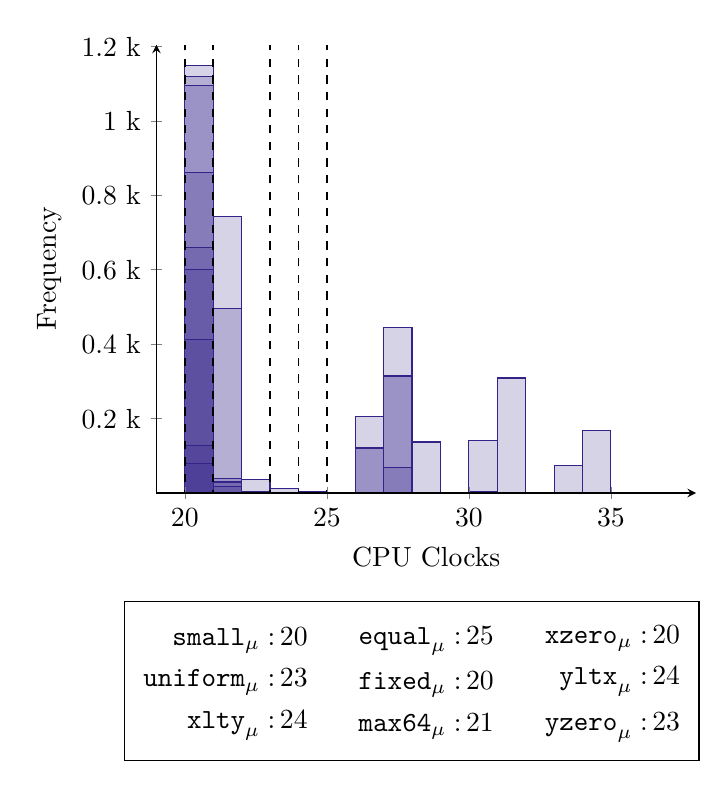
\begin{tikzpicture}[>=latex]
        \begin{axis}[
            axis x line=center,
            axis y line=center,
            name=ax,
            scaled y ticks=base 10:-3,
            ytick scale label code/.code={},
            yticklabel={\pgfmathprintnumber{\tick} k},
            xlabel={CPU Clocks},
            ylabel={Frequency},
            x label style={at={(axis description cs:0.5,-0.1)},anchor=north},
            y label style={at={(axis description cs:-0.1,.5)},rotate=90,anchor=south,yshift=4mm},
            area style,
            ymin=0,
            xmin=19,
            xmax=38,
            ymax=1205
            ]
            \addplot+ [ybar interval,mark=no,color=firstCol,fill=firstCol,fill opacity=0.2] table {
                20 78
21 496
22 35
23 1
24 0
25 0
26 1
27 0
28 0
29 0
30 141
31 309
32 0
33 0
34 1
35 0
36 1
37 1
            };
\addplot+ [ybar interval,mark=no,color=firstCol,fill=firstCol,fill opacity=0.2] table {
                20 1119
21 8
            };
\addplot+ [ybar interval,mark=no,color=firstCol,fill=firstCol,fill opacity=0.2] table {
                20 861
21 17
22 3
23 0
24 0
25 0
26 0
27 69
28 137
29 0
30 1
31 0
32 0
33 0
34 0
35 0
36 0
37 1
            };
\addplot+ [ybar interval,mark=no,color=firstCol,fill=firstCol,fill opacity=0.2] table {
                20 1148
21 10
            };
\addplot+ [ybar interval,mark=no,color=firstCol,fill=firstCol,fill opacity=0.2] table {
                20 659
21 29
22 3
23 0
24 1
25 0
26 122
27 314
28 1
29 1
30 3
31 0
32 0
33 0
34 0
35 0
36 0
37 2
            };
\addplot+ [ybar interval,mark=no,color=firstCol,fill=firstCol,fill opacity=0.2] table {
                20 413
21 39
22 1
23 0
24 3
25 0
26 205
27 445
28 2
29 1
30 0
31 0
32 0
33 0
34 0
35 1
36 0
37 1
            };
\addplot+ [ybar interval,mark=no,color=firstCol,fill=firstCol,fill opacity=0.2] table {
                20 1094
21 11
            };
\addplot+ [ybar interval,mark=no,color=firstCol,fill=firstCol,fill opacity=0.2] table {
                20 128
21 743
22 0
23 13
24 3
25 0
26 0
27 0
28 1
29 2
30 0
31 0
32 0
33 75
34 169
35 0
36 0
37 2
            };
\addplot+ [ybar interval,mark=no,color=firstCol,fill=firstCol,fill opacity=0.2] table {
                20 600
21 32
22 1
23 1
24 1
25 0
26 120
27 315
28 1
29 0
30 1
31 1
32 0
33 0
34 0
35 0
36 0
37 2
            };
                                \draw[color=black, line width=0.2mm, dashed] 
                (axis cs:25, -60.25) -- (axis cs:25, 1205);
                \draw[color=black, line width=0.2mm, dashed] 
                (axis cs:20, -60.25) -- (axis cs:20, 1205);
                \draw[color=black, line width=0.2mm, dashed] 
                (axis cs:21, -60.25) -- (axis cs:21, 1205);
                \draw[color=black, line width=0.2mm, dashed] 
                (axis cs:20, -60.25) -- (axis cs:20, 1205);
                \draw[color=black, line width=0.2mm, dashed] 
                (axis cs:23, -60.25) -- (axis cs:23, 1205);
                \draw[color=black, line width=0.2mm, dashed] 
                (axis cs:24, -60.25) -- (axis cs:24, 1205);
                \draw[color=black, line width=0.2mm, dashed] 
                (axis cs:20, -60.25) -- (axis cs:20, 1205);
                \draw[color=black, line width=0.2mm, dashed] 
                (axis cs:24, -60.25) -- (axis cs:24, 1205);
                \draw[color=black, line width=0.2mm, dashed] 
                (axis cs:23, -60.25) -- (axis cs:23, 1205);
        \end{axis} 
        \node[below=15mm of ax] (1) {
            $\begin{aligned}
                \texttt{equal}_\mu: & \,25\\
                \texttt{fixed}_\mu: & \,20\\
                \texttt{max64}_\mu: & \,21
            \end{aligned}$
        };
        \node[left=4mm of 1] (2) {
            $\begin{aligned}
                \texttt{small}_\mu: & \,20\\
                \texttt{uniform}_\mu: & \,23\\
                \texttt{xlty}_\mu: & \,24
            \end{aligned}$
        };
        \node[right=4mm of 1] (3) {
            $\begin{aligned}
                \texttt{xzero}_\mu: & \,20\\
                \texttt{yltx}_\mu: & \,24\\
                \texttt{yzero}_\mu: & \,23
            \end{aligned}$
        };
        \node[fit=(1)(2)(3),draw]{};
        \end{tikzpicture}%
      \end{lrbox}\resizebox{\textwidth}{!}{\usebox{\mybox}}
      \caption{Fuzzing results visualized. The means of each fuzz class are shown as vertical lines.}
    \end{subfigure}
    \hspace{1cm}
    \begin{subfigure}[b]{0.3\textwidth}
      \begin{lstlisting}[style=defstyle,language={[x86masm]Assembler},basicstyle=\footnotesize\ttfamily,breaklines=true]
...
  pushq	%rbp
  movq	%rsp, %rbp
  movq	%rdi, -8(%rbp)
  movq	%rsi, -16(%rbp)
  cmpq	$0, -8(%rbp)
  js	.L2
  movl	$-29, %eax
  movl	$-37, %edx
  movl	%eax, %ecx
  sarl	%cl, %edx
  movl	%edx, %eax
  cmpl	$1, %eax
  jle	.L3
.L2:
  movl	$1, %eax
  jmp	.L5
.L3:
  movl	$0, %eax
.L5:
  popq	%rbp
  ret
...\end{lstlisting} 
       \caption{Fuzzed assembly code.}
  \end{subfigure}
  \caption{An example of a true positive, i.e. a variable-time program that was rejected by Welch's t-test, from the \texttt{O0} dataset. 
  The source code of the program is shown in Appendix \ref{appendix:general-optimizations-results}. 
  Notice that inputs from the input classes \texttt{small}, \texttt{xzero}, \texttt{fixed} and \texttt{max64} are significantly faster than the rest.
  That is because the program branches on whether $x$ is signed or not (\texttt{js} instruction in line 7), which it never is in these 4 classes.}
  \label{fig:general-optimizations-O0-true-positive}
\end{figure}

Findings from the other datasets also deserve mentioning.
The \texttt{O1}, \texttt{O2}, \texttt{O3} and \texttt{Os} datasets had several false negatives, i.e. programs that were not rejected by Welch's t-test, but were variable-time.
Concretely, we saw examples where the assembled code branched on a \textit{very} specific scenario, e.g. if $x = 8129346172934691$, which is near-impossible to detect by fuzzing since the probability of hitting that specific value is very low.
We did not find any false positives in any other dataset than \texttt{O0}.
This is because the vast majority of programs in the \texttt{O1}, \texttt{O2}, \texttt{O3} and \texttt{Os} datasets were variable-time.
This points to the fact that more aggressive optimizations that introduce conditional branching are more likely to produce actual variable-time machine code.
The reason that Welch's t-test did not detect vulnerabilities in all programs in the datasets is likely due to the above-mentioned false negatives, but also because the t-test has some inherent limitations as mentioned in Section \ref{sec:statistical-analysis}.
Concrete examples of true and false positives and negatives can be found in Appendix \ref{appendix:general-optimizations-results}.

Finally, we want to address the fact that the general optimizations datasets were generated with programs that had ASTs of max depth 5.
This was done to reduce the length of the programs to make them more manageable for analysis.
However, we also generated datasets with ASTs of max depth 12 and found that the results were similar in the \texttt{O0} and \texttt{O1} datasets, while the \texttt{O2}, \texttt{O3} and \texttt{Os} datasets had significantly more programs with conditional branching -- around 5\%, 5\% and 2\% respectively.
We deem the choice of max depth 5 to be a good compromise between the length of the programs and the number of conditional branches since our results underline the problem we are trying to address.

\subsection{Specific Optimizations}
\label{sec:specific-optimizations}
The results in Table \ref{tab:general-optimizations} show that the percentage of vulnerable programs is the highest for the \texttt{O0} dataset, then it decreases significantly for the \texttt{O1} dataset, and then it increases significantly for the \texttt{O2} and \texttt{O3} datasets.
The significant decrease from \texttt{O0} to \texttt{O1} points to the fact that some optimizations in \texttt{gcc} decrease the number of conditional branches. 
Despite running several hundred experiments testing each possible configurable optimization flag \citep{gcc-manual} individually, we were not able to identify which optimizations were responsible for this decrease.
Furthermore, applying all configurable optimizations from \texttt{O1} to \texttt{O0} at once did not result in a decrease in the number of conditional branches.
This points to the fact that the responsible optimizations are non-configurable, i.e. they are always enabled for \texttt{O1}.
This also underlines the fact that all the \texttt{O*} flags enable optimizations that are non-configurable \citep{gcc-manual}, which in turn gives the developer less control over disabling problematic optimizations to increase the security of the code.

The significant increase from \texttt{O1} to \texttt{O2} and \texttt{O3} points to the fact that some optimizations in \texttt{gcc} can introduce conditional branches and therefore timing vulnerabilities. 
We identified a configurable compiler optimization that was responsible for introducing conditional branches in our datasets: \texttt{ftree-pre}.
This optimization performs partial redundancy elimination \citep{gcc-manual}.
\texttt{ftree-pre} is enabled by default for \texttt{O2}, \texttt{O3}, and \texttt{Os}, but not for \texttt{O1}.

Partial redundancy elimination (PRE) is a form of common subexpression elimination (CSE) that tries to eliminate redundant computations. 
We discussed how CSE works and how it can introduce conditional branches in Section \ref{sec:cse}.
Specifically, PRE tries to eliminate computations that are redundant in some, but not all, control flow paths.
This is done by moving the computation to a point in the program where it is guaranteed to be executed only once.
This results in different control flow paths with different amounts of instructions, which in turn result in timing vulnerabilities.

\subsection{Vulnerable Expressions}
\label{sec:vulnerable-expressions}
Finally, we identified various types of expressions that were compiled into conditional branches.
We identified expressions on the form $c$ \texttt{op} $x$ \texttt{comp} $y$, where $c$ is a constant, \texttt{op} is a bitwise operator, \texttt{comp} is a comparison operator, and $x$ and $y$ are variables.
Expressions of this form result in constant-time code containing conditional branches, much like the example in Figure \ref{fig:assembly-inspection-example}.

A more severe type of expression that we identified was expressions on the form $undefined$ \texttt{op} $(x$ \texttt{comp} $y)$, where $undefined$ contains undefined behavior, \texttt{op} is a bitwise operator, \texttt{comp} is a comparison operator, and $x$ and $y$ are variables. 
Expressions of this form sometimes result in variable-time code when compiled with \texttt{O0}.
However, when compiled with \texttt{O1}, \texttt{O2}, \texttt{O3} or \texttt{Os}, the entire program is optimized away and replaced with \texttt{return 0;}.
This is because the compiler can deduce that the expression contains undefined behavior, and, according to the C standard, the compiler is allowed to replace undefined behavior with anything \citep{c-standard}.
An example of this type of expression and its corresponding assembly, when compiled with \texttt{O0}, is shown in Figure \ref{fig:vulnerable-expression}.

\begin{figure}[H]
  \centering
     \begin{subfigure}[b]{0.41\textwidth}
        \begin{lstlisting}[style=defstyle,language={C},basicstyle=\ttfamily,breaklines=true]
int program(long long int x, long long int y) { 
  return (42 >> -1) & (x == y); 
}\end{lstlisting} 
      \vspace{6em}
      \caption{An example of a program containing an expression of the form $undefined$ \texttt{op} $(x$ \texttt{comp} $y)$.
      Specifically, bit-shifting with a negative number is undefined behavior in C \citep{c-standard}.}
    \end{subfigure}
    \hspace{1cm}
    \begin{subfigure}[b]{0.3\textwidth}
      \begin{lstlisting}[style=defstyle,language={[x86masm]Assembler},basicstyle=\footnotesize\ttfamily,breaklines=true]
...
  pushq   %rbp
  movq    %rsp, %rbp
  movq    %rdi, -8(%rbp)
  movq    %rsi, -16(%rbp)
  movq    -8(%rbp), %rax
  cmpq    -16(%rbp), %rax
  jne     .L2
  movl    $-1, %eax
  movl    $42, %edx
  movl    %eax, %ecx
  sarl    %cl, %edx
  movl    %edx, %eax
  andl    $1, %eax
  jmp     .L4
.L2:
  movl    $0, %eax
.L4:
  popq    %rbp
  ret
...\end{lstlisting} 
       \caption{Corresponding assembly code when compiled with \texttt{O0} in \texttt{gcc}.}
  \end{subfigure}
  \caption{An example of a small program that causes \texttt{gcc} to generate variable-time code when compiled with \texttt{O0}. Specifically, one can obtain whether $x$ is equal to $y$ by timing the program.}
  \label{fig:vulnerable-expression}
\end{figure}

Finally, and perhaps most importantly, we identified expressions that will result in variable-time code when compiled with \texttt{O2}, \texttt{O3} and \texttt{Os}.
As mentioned in Section \ref{sec:specific-optimizations}, partial redundancy elimination (PRE) can introduce conditional branches.
PRE is enabled for \texttt{O2}, \texttt{O3} and \texttt{Os} \citep{gcc-manual}.
In some expressions of the form $e$ \texttt{comp} $e'$, where $e$ and $e'$ contain subexpressions that are not common between $e$ and $e'$, PRE will introduce conditional branches. An example of this is shown in Figure \ref{fig:pre-example}.

\begin{figure}[H]
  \centering
  \begin{lstlisting}[style=defstyle,language={C},basicstyle=\ttfamily,breaklines=true, xleftmargin=3cm, xrightmargin=3cm]
int program(long long int x, long long int y) { 
  return 42 * (x == 42) == (y == 42); 
}\end{lstlisting} 
    \caption{An example of a program that will be variable-time when compiled with \texttt{O2}, \texttt{O3} or \texttt{Os}, specifically because of PRE.
    PRE will identify two control flow paths in this expression: 
    One where $x=42$ and one where $x \neq 42$.
    If $x=42$, the expression will always evaluate to $0$ since \texttt{42 * (42 == 42) == (y == 42)} will evaluate to $42 \stackrel{?}{=} 0$ or $42 \stackrel{?}{=} 1$ which is false in both cases.
    If $x \neq 42$, the expression depends on whether $y=42$.
    Hence \texttt{(y == 42)} is redundant in the first control flow path, but not in the second.
    As a result, PRE will insert a conditional branch that branches on $x = 42$ and only considers $y$ if that is \textit{not} the case.}
    \label{fig:pre-example}
\end{figure}


\section{Evaluation}
\todo{Evaluation of OptiFuzz and analysis. Is it accurate?}

\todo{From results, we can see that most programs with conditional branches are rejected by the t-test.
This means that our underapproximation by the inspection is okay.}

\section{Discussion}
From the previous sections, it is clear that modern compilers introduce timing vulnerabilities in constant-time programs.
This is devastating for security since it means that developers cannot reliably write constant-time code.
A solution is required.
In this section, we discuss how the problem can be solved and what the implications different solutions have on security and efficiency.

As shown in Section \ref{sec:gcc-vs-clang}, \texttt{clang} is much more conservative when it comes to inserting conditional branches in constant-time programs.
Instead of inserting variable-time conditional branches, \texttt{clang} uses constant-time conditional moves to implement branching control flow.
From this observation, it might be tempting to conclude that always substituting conditional branches with conditional moves is the solution to the problem.
However, there is more to the story.

\texttt{cmov} instructions severely restrict the out-of-order engine on modern CPUs since \texttt{cmov} instructions increase the data dependency between instructions significantly \citep{intel-optimization-reference}. 
Furthermore, branch predictions are not used for \texttt{cmov} instructions, which can lead to significant performance degradation.
Hence, we have to address this trade-off between security and efficiency.

\subsection{Forcing \texttt{cmov} Instructions When Necessary}
This trade-off between security and efficiency has led multiple researchers to propose solutions that only force \texttt{cmov} instructions to be used on critical data \citep{what-you-c,llvm-issues-blog-post}.
In both studies, the authors propose to add the possibility to specify forced \texttt{cmov} instructions in the source code and restrict the backend of the compiler to not being able to optimize the \texttt{cmov} away for those specific instructions.
This solution has the advantage that it does not affect the performance of non-critical parts of the program.
In fact, \citeauthor{what-you-c} show that their solution only introduces a performance penalty of 1\% and sometimes even increases performance.

However, this solution also has its disadvantages.
First, the solution relies heavily on the developer.
The developer has to know which parts of the program are critical, and also be able to use the language extension correctly.
In turn, it means that security relies on human factors, which are error-prone.
Second, the solution relies on the compiler being configurable to avoid forced \texttt{cmov} instructions being optimized away.
As we discussed in Section \ref{sec:gcc-vs-clang} and \ref{sec:general-optimizations}, \texttt{clang} seems to be quite configurable while \texttt{gcc} does not.
Hence, the solution might not be easily applicable to all compilers.

Another solution is to implement vulnerable parts of the program using a domain-specific language that is designed to be constant-time.
\citeauthor{fact} proposed a domain-specific language, called FaCT, for implementing constant-time cryptographic algorithms \citep{fact}.
FaCT is designed to be interoperable with C, and the compiler ensures constant-time code by leveraging the \texttt{ct-verif} tool that is based on verification of the LLVM IR \cite{verifying-constant-time-llvm}.
\texttt{ct-verif} operates on a formalization of constant-time code and verifies based on a theoretically sound and complete methodology.
However, \citeauthor{verifying-constant-time-llvm} note that the verification process of \texttt{ct-verif} is not guaranteed to identify all timing vulnerabilities due to translation between the LLVM IR and machine code, and due to possible incompleteness of their formalization of constant-time code. 
Some of these issues were experimentally verified.
However, generally \texttt{ct-verif} captures significantly more timing vulnerabilities than other verification alternatives \citep{verifying-constant-time-llvm}.
Additionally, \texttt{ct-verif} is efficient at verifying constant-time code, often being much faster than the compilation step, but occasionally being a few times slower.

\subsection{Bullet-proofing the Compiler}
A more radical approach is to force the compiler to always produce constant-time code.
\citeauthor{verified-constant-time-c-comiler} provides a formally verified constant-time C compiler, built on top of the CompCert verified C compiler \citep{verified-constant-time-c-comiler}. 
The constant-time CompCert compiler guarantees that constant-time source code is compiled into constant-time machine code.
This is achieved by instrumenting the operational semantics of CompCert's IR to be able to capture cryptographic constant-time and proving that cryptographic constant-time is preserved during compilation. 
This has immense advantages for security.

However, the security advantages come at the cost of efficiency. 
The constant-time CompCert compiler is significantly slower than \texttt{gcc}.
Experimental results show an efficiency penalty of well over 100\% in some cases \citep{verified-constant-time-c-comiler}.

\subsection{Testing Solutions}
The final category of solutions we identified is black-box testing solutions like DudeCT \citep{dudect} and our tool OptiFuzz.
Concretely, one can test specific implementations for timing vulnerabilities using these tools.
These tests can even be automated to run as part of a continuous integration pipeline.
Solutions in this category have the obvious advantage that they are simple and require no modeling of hardware behavior or language semantics.
It is arguably the most practical solution since it does not require any changes to the compiler or the language.
It also does not induce any performance penalty.

The testing solutions, however, come with a significant security disadvantage in that they are noisy and not exact.
As we showed in Section \ref{sec:general-optimizations}, OptiFuzz will produce false positives and false negatives.
\citeauthor{dudect} raised similar concerns for DudeCT.
Fuzzing tools provide more of an indication of the presence of timing vulnerabilities than a guarantee.

\todo{Argue that many solutions exist with a mixture of security and efficiency.
We argue that people should start using them.
Perhaps OptiFuzz + compromise solutions}

\section{Conclusion and Future Work}
We have a lot of ideas for future work that we did not get around to. These include:
\begin{itemize}
    \setlength\itemsep{-0.6em}
    \item Extend OptiFuzz to generate more complicated programs, eg. by reintroducing the division and modulus operators while dealing with division by zero in a meaningful way.
    \item Increasing the precision of the assembly inspection. One way could be to detect if branches contain the same amount of work and identify them as constant time.
    \item Implement other relevant input classes. A dynamic class containing the hardcoded values from a program. This might be able to catch the very specific but unpredictable values that courses branching.
    \item Extending the usage of Welsh's t-test to all classes, and not just between \texttt{uniform} and \texttt{fixed}.
    \item Create a tool that warns developers in real-time about constant C expressions that might be compiled to variable time by comparing it to a database precomputed using OptiFuzz. This tool could furthermore be implemented in a CI/CD environment.
    \item Extend OptiFuzz to support other processor architecture, especially including ones used by embedded systems.
\end{itemize}


\pagebreak

\bibliographystyle{abbrvnat}
\bibliography{litterature}

\pagebreak
\begin{appendices}

\section{Select General Optimizations Results}
\label{appendix:general-optimizations-results}
%\documentclass[10pt]{article}
\input{prelude}
\usepackage[authoryear]{natbib}

\title{
  Optimizing Away Security in C
}

\groupNumber{10}
\author{Anders B. Clausen \and Johan T. Degn \and Jonathan Eilath}

\begin{document}
\maketitle
\thispagestyle{empty}

\section*{Abstract}
\todo{After the paper is done}

\section{Introduction}
\input{chapters/introduction.tex}

\section{Preliminaries}
\input{chapters/preliminaries.tex}

\section{OptiFuzz}
\input{chapters/optifuzz.tex}
\subsection{Code Generation}
\input{chapters/code-generation.tex}
\subsection{Assembly Inspection}
\input{chapters/assembly-inspection.tex}
\subsection{Fuzzing}
\input{chapters/fuzzing.tex}
\subsection{Statistical Analysis}
\input{chapters/statistical-analysis.tex}

\section{Experimental Results}
\input{chapters/results.tex}

\section{Evaluation}
\input{chapters/evaluation.tex}

\section{Discussion}
\input{chapters/discussion.tex}

\section{Conclusion and Future Work}
\input{chapters/conclusion.tex}

\pagebreak

\bibliographystyle{abbrvnat}
\bibliography{litterature}

\pagebreak
\begin{appendices}

\section{Select General Optimizations Results}
\label{appendix:general-optimizations-results}
%\input{appendix/general-optimizations-results/master.tex}

\end{appendices}

\end{document}

\end{appendices}

\end{document}

\end{appendices}

\end{document}

\end{appendices}

\end{document}